\section{Experimentos e Resultados}\label{sec:experimentos}

Nas proximas seções, apresentamos os experimentos conduzidos para avaliar o desempenho do \gls{CLAIRE} na análise de modelos de agrupamento provenientes de diferentes famílias de algoritmos. O objetivo é investigar como o método se comporta em cenários variados, tanto em termos de estrutura dos dados quanto de diversidade dos modelos avaliados.

Para isso, utilizamos um conjunto heterogêneo de bases de dados (ilustradas na \ref{fig:datasets}), composto por três conjuntos clássicos amplamente utilizados na literatura, sendo eles o Iris (4 atributos, $N = 150$), Wine (13 atributos, $ N = 178$) e Breast Cancer (30 atributos,  $N=569$). Além de seis conjuntos sintéticos gerados conforme exemplos disponibilizados na documentação do Scikit-learn: Aniso (três gaussianas anisotrópicas), Blobs (três gaussianas isotrópicas e bem separadas), Varied (três gaussianas com variâncias distintas), Noisy Moons (duas luas interligadas), Noisy Circles (dois círculos concêntricos) e No Structure (pontos distribuídos uniformemente).

\begin{figure}[t]
    \centering
    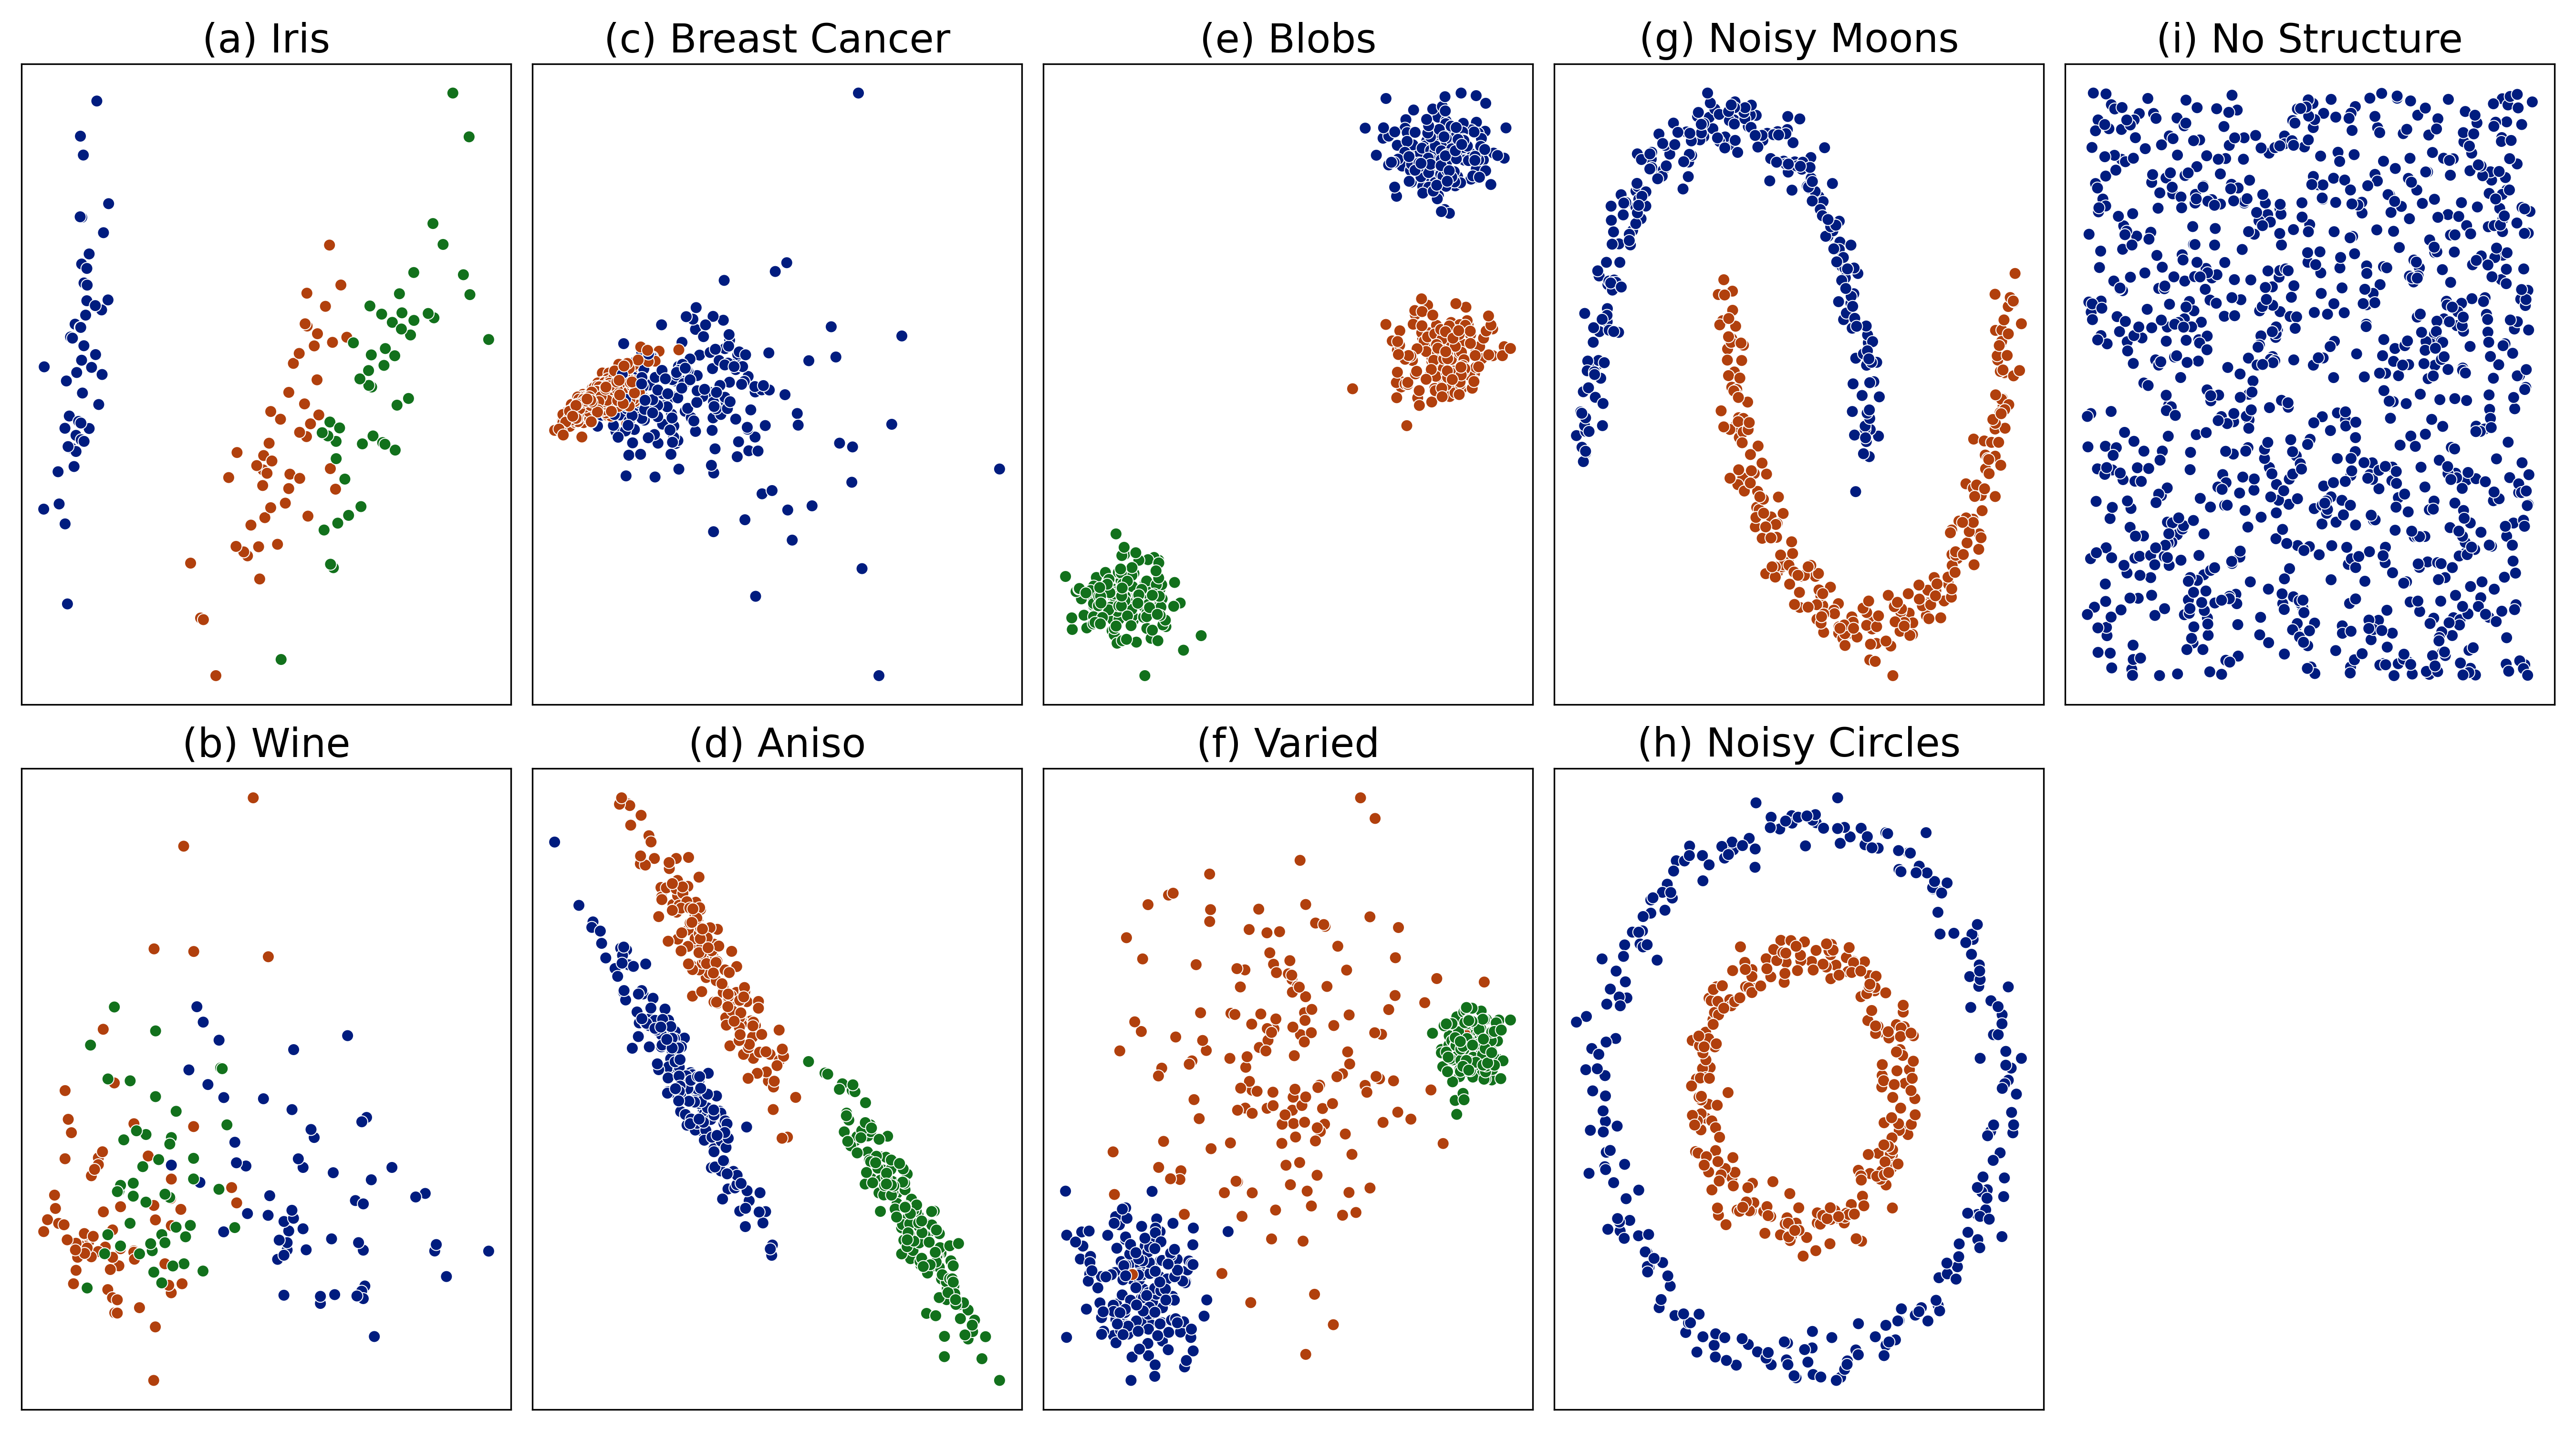
\includegraphics[width = 1\textwidth]{chapters/fundamentacao/imagens/dataset_distribution_labels_row.png}
    \caption{Conjunto de dados usado nos experimentos. Para os conjuntos reais (Iris, Wine e Breast Cancer), os primeiros dois componentes estâo sendo mostrados. Conjuntos de dados sintéticos pode ser encontrados na documentação do scikit-learn \cite{scikit-learn-example}}
    \label{fig:datasets}
\end{figure}

A escolha desses conjuntos de dados buscou contemplar diferentes padrões estruturais frequentemente encontrados em aplicações reais, incluindo clusters aproximadamente esféricos, estruturas não lineares, variações de densidade e ausência de estrutura clara de agrupamento. Ao mesmo tempo, esses cenários permitem uma análise interpretável dos resultados, pois é possível antecipar quais tipos de algoritmos tendem a se ajustar melhor a cada configuração. Para os conjuntos sintéticos, foram amostradas 500 instâncias por base, enquanto para as bases reais e para o conjunto No Structure utilizamos 1000 instâncias.

Nos experimentos, empregamos seis algoritmos de clustering amplamente reconhecidos e utilizados na literatura. A seleção desses métodos foi realizada de modo a abranger diferentes pressupostos modelais e critérios de otimização, o que naturalmente conduz a partições distintas para um mesmo conjunto de dados. Essa diversidade é fundamental para o \gls{CLAIRE}, uma vez que o método se apoia na variação e na concordância entre modelos para estimar habilidades e dificuldades latentes. Como consequência, os modelos produzidos não são diretamente comparáveis por meio de um único índice interno tradicional.


\begin{table*}[!htb]

    \centering
    \caption{Valores dos hiperparâmetros para cada um dos seis métodos de agrupamento. O OPTICS utilizou hiperparâmetros padrão para conjuntos de dados reais e configurações específicas extraídas da documentação do Scikit-learn para cada conjunto de dados sintéticos; consulte o Apêndice para obter detalhes.}
    \begin{tabular}{ll}
    \toprule
       Algoritmo  & Hiperparâmetro\\
    \midrule
       K-means  & $K \in \{1, 2, 3, 4, 5, 6, 7, 8\}$\\
       Kernel K-means  & $K \in \{1, 2, 3, 4, 5, 6, 7, 8\}$\\
       DBSCAN  & $\epsilon \in \{0.1, 0.2, 0.3,0.4, 0.5, 0.6, 0.7, 0.8, 0.9\}$\\
       Spectral Clustering  & $K \in \{1, 2, 3, 4, 5, 6, 7, 8\}$, affinity=\textsf{nearest\_neighbors}\\
       Mean Shift  & -\\
       OPTICS  & Veja a legenda\\
    \midrule
    \end{tabular}
    \label{tab:hyperparams}
    
    % Hyperparameter values for each of the six clustering methods. OPTICS used default hyperparameters for real datasets and specific configurations taken from Scikit-learn's documentation for each synthetic dataset, see the Appendix for details.
    % }
   % \label{tab:alg:hyper}
\end{table*}

A Tabela \ref{tab:hyperparams} apresenta os algoritmos considerados e os valores de hiperparâmetros explorados, totalizando 35 modelos distintos para cada conjunto de dados. Todos os parâmetros não especificados foram mantidos nos valores padrão da implementação do Scikit-learn, com exceção do Kernel K-means, ajustado utilizando a biblioteca tslearn \cite{tslearn}.

Os experimentos foram organizados em quatro etapas principais. Inicialmente, utilizamos o \gls{CLAIRE} para ranquear os modelos e estimar as dificuldades das instâncias. Em seguida, analisamos a correlação entre as habilidades estimadas pelo \gls{CLAIRE} e diferentes índices tradicionais de validação de clustering. Posteriormente, investigamos o impacto da inclusão de partições aleatórias no conjunto de modelos. Por fim, avaliamos a estabilidade das habilidades estimadas quando a composição do conjunto de modelos é alterada.


\section{Ranqueamento de modelos e avaliação de instâncias}\label{sec:ranquemaento}

Dado um conjunto de dados, cada algoritmo foi usado para agrupar o dado com cada hiperparâmetro especificado na tabela \ref{tab:hyperparams}. Então, é aplicado a equação \ref{eq:response_matrix} para gerar a resposta para cada par instância-modelo. Dessa forma, é adicionado dois modelos hipoteticos para a matriz de respostas, sendo tratados como modelos base, sendo definidos abaixo.

\begin{itemize}
    \item[1] A resposta média para cada instância, entitulado como \textit{Average Response};
    \item[2] A máxima resposta para cada instância, entitulado como \textit{Best Response}.
\end{itemize}

Ambos modelos tem como objetivo tentar capiturar a media e o melhor resultado entre os $35$ modelos avaliados. O \textit{Average Response} representa um modelo que deve retornar uma resposta média entre um grupo de 35 modelos, enquanto o \textit{Best Response} representar um modelo hipotetico equivalente a sempre retornar o modelo com a melhor resposta observada, entre os $35$ modelos, o qual deve produzir um limite superior para a performance. Assim, para cada conjunto de dados, é gerado uma matriz $M \times N$, tomando $M = 37$ ($35$ modelos com diferentes hiperparâmetros e $2$ modelos artificiais) e $N$ é o número de instâncias do conjunto de dados.

\begin{table*}[!htbp]
    \centering
    \caption{Pseudo-$R^2$ \cite{ferreirajunior2023beta4irtnewbeta3irtenhanced} e coeficinete correlação de Pearson entre observado e resposta estimada para cada conjunto de dados. Todas os coeficientes de correlação foram estatísticamente significantes ($p-value < 0.05$).}
    \begin{tabular}{lcc}
    \toprule
    Conjunto de Dados & Pseudo$-R^{2}$ & $\rho$ \\
    \midrule
    Noisy Circles & 0.943 & 0.971 \\
    Noisy Moons & 0.905 & 0.951 \\
    Varied & 0.862 & 0.928 \\
    Blobs & 0.851 & 0.922 \\
    Aniso & 0.845 & 0.919 \\
    No Structure & 0.819 & 0.905 \\
    Iris & 0.815 & 0.903 \\
    Wine & 0.684 & 0.827 \\
    Breast\_cancer & 0.576 & 0.759 \\
    \bottomrule
    \end{tabular}
    \label{tab:pseudor2_results}
\end{table*}


Considerando a matriz de resposta como entrada, o $\beta^4$-\gls{IRT} é usado para estimar a habilidade de cada modelo, e também para cada item, as dificuldades e discriminantes. Antes de seguir com a analise dos parâmetros dos modelos, é estimado um \textit{goodness-of-fit} para o $\beta^4$-\gls{IRT} para cada um dos conjuntos de dados, calculando o Pseudo-$R^2$ \cite{ferreirajunior2023beta4irtnewbeta3irtenhanced}. Assim como mostrado na tabela \ref{tab:pseudor2_results}, temos que altos valores foram obtidos pelo Pseudo-$R^2$, assim indicando  um bom ajusto entre as respostas observadas e estimadas, para todos os conjuntos de dados. Além disso, a tabela \ref{tab:pseudor2_results} traz a correlação de Pearson ($\rho$), sendo todos fortemente positivos e estatisticamente significantes ($p-value < 0.05$).

Ápos isso, dado o bom ajuste do modelo $\beta^4$-\gls{IRT}, foi ranqueado os modelos de agrupamento pelas suas habilidades estimadas para cada conjunto, como visto pela tabela  \ref{tab:abilities_iris_wine_bc} e \ref{tab:abilities_aniso_blobs_varied_moons_circles_no_structure}. Como era esperado, o \textit{Best Response}, em nenhum conjunto de dados, ele foi considerado o pior modelo.



\begin{table*}[h]
    \centering
    \tiny
    \caption{Habilidade dos modelos e ranqueamento para os conjuntos Iris, Wine e Breast Cancer. Os melhores modelos ranqueados (com exceção do \textit{Best Response}) estão marcados em \textbf{negrito}.}
        \begin{tabular}{l|c|lll}
\midrule
Modelo & Versão &  Iris & Wine & Breast Cancer \\
\midrule
Best Response &  & $0.530_{1.0}$ & $0.549_{1.0}$ & $0.550_{1.0}$ \\
\midrule
Average Response &  & $0.472_{29.0}$ & $0.501_{26.0}$ & $0.491_{21.0}$ \\
\midrule
Mean Shift &  & $0.507_{14.5}$ & $0.502_{25.0}$ & $0.525_{7.0}$ \\
\midrule
\multirow[t]{6}{*}{Optics} & - & $0.395_{33.0}$ & $0.499_{27.0}$ & $0.517_{8.0}$ \\
\midrule
\multirow[t]{9}{*}{DBSCAN} & $\epsilon=0.1$ & $0.328_{34.0}$ & $0.503_{18.5}$ & $0.515_{14.5}$ \\
 & $\epsilon=0.2$ & $0.403_{32.0}$ & $0.503_{18.5}$ & $0.515_{14.5}$ \\
 & $\epsilon=0.3$ & $0.447_{31.0}$ & $0.503_{18.5}$ & $0.515_{14.5}$ \\
 & $\epsilon=0.4$ & $0.471_{30.0}$ & $0.503_{18.5}$ & $0.515_{14.5}$ \\
 & $\epsilon=0.5$ & $0.496_{23.5}$ & $0.503_{18.5}$ & $0.515_{14.5}$ \\
 & $\epsilon=0.6$ & $0.505_{17.0}$ & $0.503_{18.5}$ & $0.515_{14.5}$ \\
 & $\epsilon=0.7$ & $0.509_{10.5}$ & $0.503_{18.5}$ & $0.515_{14.5}$ \\
 & $\epsilon=0.8$ & $0.510_{8.5}$ & $0.503_{18.5}$ & $0.515_{14.5}$ \\
 & $\epsilon=0.9$ & $0.510_{8.5}$ & $0.503_{18.5}$ & $0.515_{14.5}$ \\
\midrule
\multirow[t]{8}{*}{K-means} & $K=1$ & $0.325_{36.0}$ & $0.503_{18.5}$ & $0.515_{14.5}$ \\
 & $K=2$ & $0.507_{14.5}$ & $0.532_{6.0}$ & $0.547_{3.0}$ \\
 & $K=3$ & $0.519_{5.0}$ & $0.544_{3.0}$ & $0.542_{4.5}$ \\
 & $K=4$ & $0.512_{6.0}$ & $0.531_{7.0}$ & $0.542_{4.5}$ \\
 & $K=5$ & $0.508_{12.0}$ & $0.517_{10.0}$ & $0.487_{23.0}$ \\
 & $K=6$ & $0.497_{22.0}$ & $0.525_{8.0}$ & $0.478_{25.0}$ \\
 & $K=7$ & $0.500_{20.0}$ & $0.509_{11.0}$ & $0.463_{27.5}$ \\
 & $K=8$ & $0.495_{25.0}$ & $0.491_{29.0}$ & $0.463_{27.5}$ \\
\midrule
\multirow[t]{8}{*}{Kernel K-means} & $K=1$ & $0.325_{36.0}$ & $0.503_{18.5}$ & $0.515_{14.5}$ \\
 & $K=2$ & $0.507_{14.5}$ & $0.484_{31.0}$ & $0.483_{24.0}$ \\
 & $K=3$ & $\mathbf{0.523_{2.5}}$ & $0.467_{32.0}$ & $0.439_{33.0}$ \\
 & $K=4$ & $0.509_{10.5}$ & $0.466_{33.5}$ & $0.450_{31.0}$ \\
 & $K=5$ & $0.504_{18.5}$ & $0.466_{33.5}$ & $0.431_{34.0}$ \\
 & $K=6$ & $0.498_{21.0}$ & $0.455_{35.0}$ & $0.421_{36.0}$ \\
 & $K=7$ & $0.496_{23.5}$ & $0.441_{37.0}$ & $0.418_{37.0}$ \\
 & $K=8$ & $0.490_{27.0}$ & $0.444_{36.0}$ & $0.425_{35.0}$ \\
\midrule
\multirow[t]{8}{*}{Spectral Clustering} & $K=1$ & $0.325_{36.0}$ & $0.503_{18.5}$ & $0.515_{14.5}$ \\
 & $K=2$ & $0.507_{14.5}$ & $0.538_{4.5}$ & $\mathbf{0.549_{2.0}}$ \\
 & $K=3$ & $\mathbf{0.523_{2.5}}$ & $\mathbf{0.545_{2.0}}$ & $0.533_{6.0}$ \\
 & $K=4$ & $0.520_{4.0}$ & $0.538_{4.5}$ & $0.489_{22.0}$ \\
 & $K=5$ & $0.511_{7.0}$ & $0.519_{9.0}$ & $0.474_{26.0}$ \\
 & $K=6$ & $0.504_{18.5}$ & $0.506_{12.0}$ & $0.460_{29.0}$ \\
 & $K=7$ & $0.492_{26.0}$ & $0.493_{28.0}$ & $0.452_{30.0}$ \\
 & $K=8$ & $0.486_{28.0}$ & $0.486_{30.0}$ & $0.440_{32.0}$ \\
\midrule
\end{tabular}
\label{tab:abilities_iris_wine_bc}
\end{table*}




\begin{table*}[!t]
    \centering
    \tiny
    \caption{Habilidades e classificação dos modelos para Aniso, Blobs, Varied, Moons, Circles e No Structure. A classificação de cada modelo é mostrada em subscrito. Os modelos com melhor classificação (exceto Melhor Resposta) estão marcados em \textbf{negrito}.}
        \begin{tabular}{l|c|lllllll}
\midrule
Modelo & Versão & Aniso & Blobs & Varied & Moons & Circles & No Structure \\
\midrule
Best Response &  & $0.505_{1.0}$ & $0.505_{4.5}$ & $0.520_{1.0}$ & $0.487_{1.0}$ & $0.498_{1.0}$ & $0.518_{1.0}$ \\
\midrule
Average Response &  & $0.458_{27.0}$ & $0.420_{28.0}$ & $0.456_{26.0}$ & $0.441_{29.0}$ & $0.463_{30.0}$ & $0.476_{23.0}$ \\
\midrule
Mean Shift &  & $0.491_{9.5}$ & $\mathbf{0.505_{4.5}}$ & $\mathbf{0.517_{2.0}}$ & $0.467_{13.5}$ & $0.464_{28.5}$ & $0.449_{30.0}$ \\
\midrule
\multirow[t]{6}{*}{Optics} & - & $0.500_{4.0}$ & $\mathbf{0.505_{4.5}}$  & $0.460_{24.5}$  & $\mathbf{0.482_{4.5}}$ & $0.484_{11.5}$  & $0.449_{30.0}$ \\
\midrule
\multirow[t]{9}{*}{DBSCAN} & $\epsilon=0.1$ & $0.475_{22.0}$ & $0.494_{10.0}$ & $0.484_{21.0}$ & $0.438_{30.0}$ & $0.464_{28.5}$ & $0.434_{37.0}$ \\
 & $\epsilon=0.2$ & $0.501_{3.0}$ & $0.504_{9.0}$ & $0.504_{9.0}$ & $\mathbf{0.482_{4.5}}$ & $0.484_{11.5}$ & $0.449_{30.0}$ \\
 & $\epsilon=0.3$ & $0.396_{29.0}$ & $\mathbf{0.505_{4.5}}$ & $0.380_{28.0}$ & $\mathbf{0.482_{4.5}}$ & $0.484_{11.5}$ & $0.449_{30.0}$ \\
 & $\epsilon=0.4$ & $0.396_{29.0}$ & $\mathbf{0.505_{4.5}}$ & $0.378_{29.0}$ & $\mathbf{0.482_{4.5}}$ & $0.484_{11.5}$ & $0.449_{30.0}$ \\
 & $\epsilon=0.5$ & $0.396_{29.0}$ & $0.426_{23.0}$ & $0.376_{30.5}$ & $\mathbf{0.482_{4.5}}$ & $0.484_{11.5}$ & $0.449_{30.0}$ \\
 & $\epsilon=0.6$ & $0.395_{34.0}$ & $0.426_{23.0}$ & $0.376_{30.5}$ & $0.351_{34.0}$ & $0.395_{34.0}$ & $0.449_{30.0}$ \\
 & $\epsilon=0.7$ & $0.395_{34.0}$ & $0.426_{23.0}$ & $0.375_{34.5}$ & $0.351_{34.0}$ & $0.395_{34.0}$ & $0.449_{30.0}$ \\
 & $\epsilon=0.8$ & $0.395_{34.0}$ & $0.426_{23.0}$ & $0.375_{34.5}$ & $0.351_{34.0}$ & $0.395_{34.0}$ & $0.449_{30.0}$ \\
 & $\epsilon=0.9$ & $0.395_{34.0}$ & $0.426_{23.0}$ & $0.375_{34.5}$ & $0.351_{34.0}$ & $0.395_{34.0}$ & $0.449_{30.0}$ \\
\midrule
\multirow[t]{8}{*}{K-means} & $K=1$ & $0.395_{34.0}$ & $0.220_{36.0}$ & $0.375_{34.5}$ & $0.351_{34.0}$ & $0.395_{34.0}$ & $0.449_{30.0}$ \\
 & $K=2$ & $0.490_{11.0}$ & $0.426_{23.0}$ & $0.489_{18.0}$ & $0.464_{21.0}$ & $0.467_{27.0}$ & $0.501_{9.5}$ \\
 & $K=3$ & $0.496_{6.0}$ & $\mathbf{0.505_{4.5}}$ & $0.516_{4.0}$ & $0.467_{13.5}$ & $0.477_{22.5}$ & $0.505_{7.0}$ \\
 & $K=4$ & $0.491_{9.5}$ & $0.482_{11.5}$ & $0.515_{6.5}$ & $0.465_{18.5}$ & $0.482_{18.0}$ & $0.511_{3.0}$ \\
 & $K=5$ & $0.481_{15.5}$ & $0.456_{16.0}$ & $0.499_{10.0}$ & $0.465_{18.5}$ & $0.478_{20.5}$ & $0.503_{8.0}$ \\
 & $K=6$ & $0.481_{15.5}$ & $0.424_{27.0}$ & $0.495_{13.0}$ & $0.466_{16.0}$ & $0.475_{24.5}$ & $0.493_{13.5}$ \\
 & $K=7$ & $0.476_{20.0}$ & $0.416_{29.5}$ & $0.492_{14.0}$ & $0.459_{25.0}$ & $0.475_{24.5}$ & $0.486_{16.0}$ \\
 & $K=8$ & $0.473_{24.0}$ & $0.404_{32.0}$ & $0.486_{19.5}$ & $0.452_{28.0}$ & $0.478_{20.5}$ & $0.479_{20.5}$ \\
\midrule
\multirow[t]{8}{*}{Kernel K-means} & $K=1$ & $0.395_{34.0}$ & $0.220_{36.0}$ & $0.375_{34.5}$ & $0.351_{34.0}$ & $0.395_{34.0}$ & $0.449_{30.0}$ \\
 & $K=2$ & $0.492_{7.5}$ & $0.426_{23.0}$ & $0.490_{17.0}$ & $0.469_{12.0}$ & $0.468_{26.0}$ & $0.499_{11.5}$ \\
 & $K=3$ & $0.498_{5.0}$ & $\mathbf{0.505_{4.5}}$ & $0.516_{4.0}$ & $0.466_{16.0}$ & $0.477_{22.5}$ & $0.506_{6.0}$ \\
 & $K=4$ & $0.488_{12.5}$ & $0.482_{11.5}$ & $0.515_{6.5}$ & $0.466_{16.0}$ & $0.482_{18.0}$ & $\mathbf{0.512_{2.0}}$ \\
 & $K=5$ & $0.481_{15.5}$ & $0.457_{15.0}$ & $0.498_{11.5}$ & $0.464_{21.0}$ & $0.482_{18.0}$ & $0.501_{9.5}$ \\
 & $K=6$ & $0.481_{15.5}$ & $0.429_{18.0}$ & $0.510_{8.0}$ & $0.464_{21.0}$ & $0.488_{6.5}$ & $0.493_{13.5}$ \\
 & $K=7$ & $0.476_{20.0}$ & $0.444_{17.0}$ & $0.491_{15.5}$ & $0.460_{24.0}$ & $0.483_{15.5}$ & $0.485_{17.0}$ \\
 & $K=8$ & $0.471_{25.0}$ & $0.477_{13.0}$ & $0.498_{11.5}$ & $0.454_{26.5}$ & $0.483_{15.5}$ & $0.479_{20.5}$ \\
\midrule
\multirow[t]{8}{*}{Spectral Clustering} & $K=1$ & $0.395_{34.0}$ & $0.220_{36.0}$ & $0.375_{34.5}$ & $0.351_{34.0}$ & $0.395_{34.0}$ & $0.449_{30.0}$ \\
 & $K=2$ & $0.492_{7.5}$ & $0.358_{34.0}$ & $0.486_{19.5}$ & $\mathbf{0.482_{4.5}}$ & $0.484_{11.5}$ & $0.490_{15.0}$ \\
 & $K=3$ & $\mathbf{0.502_{2.0}}$ & $\mathbf{0.505_{4.5}}$ & $0.516_{4.0}$ & $0.477_{8.0}$ & $0.491_{4.0}$ & $0.508_{5.0}$ \\
 & $K=4$ & $0.476_{20.0}$ & $0.472_{14.0}$ & $0.491_{15.5}$ & $0.470_{10.0}$ & $\mathbf{0.493_{2.5}}$ & $0.510_{4.0}$ \\
 & $K=5$ & $0.488_{12.5}$ & $0.372_{33.0}$ & $0.465_{23.0}$ & $0.470_{10.0}$ & $\mathbf{0.493_{2.5}}$ & $0.499_{11.5}$ \\
 & $K=6$ & $0.480_{18.0}$ & $0.427_{19.0}$ & $0.469_{22.0}$ & $0.470_{10.0}$ & $0.490_{5.0}$ & $0.481_{18.0}$ \\
 & $K=7$ & $0.474_{23.0}$ & $0.416_{29.5}$ & $0.460_{24.5}$ & $0.463_{23.0}$ & $0.488_{6.5}$ & $0.480_{19.0}$ \\
 & $K=8$ & $0.470_{26.0}$ & $0.406_{31.0}$ & $0.449_{27.0}$ & $0.454_{26.5}$ & $0.487_{8.0}$ & $0.477_{22.0}$ \\
\midrule
\end{tabular}
\label{tab:abilities_aniso_blobs_varied_moons_circles_no_structure}
\end{table*}

Nos conjuntos de dados reais com três grupos (Iris e Wine), observou-se que o Spectral Clustering (no Iris) e o Kernel K-means com $K=3$ (no Wine) ocuparam as primeiras posições no ranqueamento produzido pelo \gls{CLAIRE}. Esse resultado sugere que a concordância média do conjunto de modelos tende a favorecer algoritmos que identificam corretamente o número de clusters presente nos dados. Embora o K-means com $K=3$ também tenha apresentado desempenho elevado, sua habilidade estimada foi inferior à do Spectral Clustering e do Kernel K-means. Isso pode ser explicado pelo fato de que esses dois métodos são particularmente adequados para cenários em que a separação entre grupos não é estritamente linear, característica que pode estar presente, ainda que de forma sutil, nesses conjuntos.

Para o conjunto Breast Cancer, o \gls{CLAIRE} também destacou Spectral Clustering e K-means com $K=2$ entre os modelos mais bem ranqueados. O Spectral Clustering obteve habilidade superior, possivelmente devido à sua maior capacidade de capturar estruturas de separação em espaços de dimensionalidade relativamente elevada, o que é consistente com a natureza desse conjunto de dados.

Nos conjuntos sintéticos com três clusters (Aniso, Blobs e Varied), os resultados seguiram um padrão coerente com a estrutura em que o conjunto de dados foi gerado. Para esses cenários, K-means, Kernel K-means e Spectral Clustering com o número correto de clusters foram consistentemente bem avaliados. Algoritmos que não possuem o número de clusters como hiperparâmetro explícito, como Mean Shift, OPTICS (com exceção do caso Varied) e ao menos uma configuração de DBSCAN, também recuperaram partições compatíveis com a estrutura verdadeira, refletindo altas habilidades estimadas.

Para o conjunto Aniso, todas as versões dos modelos Spectral Clustering, DBSCAN e Kernel K-Means apresentaram versões com desempenho superior ao do K-means e do Mean Shift, o que era esperado, uma vez que o K-means e o Mean Shift tendem a se ajustar bem quando o conjunto de dados consiste principalmente em clusters esféricos de tamanho semelhante. Este é o caso do conjunto de dados Blobs, para o qual Mean Shift, OPTICS, DBSCAN, K-means, Spectral Clustering e Kernel K-means empataram em primeiro lugar com o \textit{Best Response}.

Para o conjunto Varied, apesar da existência de três grupos, as diferenças nas variâncias, especialmente a maior dispersão do cluster central, geram regiões de sobreposição com os demais grupos. Dessa forma, K-means ($K=3$), Mean Shift e Kernel K-means ($K=3$) tenderam a dividir o espaço em três regiões de tamanhos comparáveis, estratégia que se mostrou competitiva segundo o \gls{CLAIRE}. O Mean Shift apresentou a maior habilidade estimada (desconsiderando o Best Response), enquanto K-means, Kernel K-means e Spectral Clustering com $K=3$ apresentaram desempenhos muito próximos entre si.

O conjunto Noisy Moons, caracterizado por duas estruturas alongadas e não linearmente separáveis, teve modelos como o DBSCAN, Spectral Clustering e OPTICS foram alocados nas primeiras posições do ranqueamento, como era esperado, como podemos ver na tabela \ref{tab:abilities_aniso_blobs_varied_moons_circles_no_structure}, com $4$ versões do DBSCAN, uma versão do Spectral Clustering e o OPTICS compartilhando o topo do ranqueamento. Esse padrão reforça a capacidade do CLAIRE de refletir a adequação estrutural dos algoritmos às características geométricas dos dados.

No caso do Noisy Circles, o \gls{CLAIRE} algumas versões de Spectral Clustering ficaram entre os melhores, enquanto Kernel K-means com $K=6$, OPTICS e algumas configurações de DBSCAN também apresentaram habilidades elevadas. Esses métodos são significativamente eficazes em cenários que existe estruturas não convexas e geometrias complexas. Ainda que o Kernel K-means não tenha identificado explicitamente o número correto de clusters, versões de Spectral Clustering com $2 \leq K \leq 8$ mantiveram alta concordância com o conjunto de modelos. Além disso, tanto o OPTICS quanto as melhores configurações de DBSCAN identificaram corretamente os dois grupos presentes nos dados, alcançando posicionamento equivalente ao Spectral Clustering com $K=2$, conforme ilustrado na Figura correspondente.

Para o conjunto Noisy Circles, o \gls{CLAIRE} posicionou algumas configurações de Spectral Clustering entre as primeiras colocações do ranqueamento, enquanto o Kernel K-means com $K=6$, o OPTICS e determinadas versões do DBSCAN também apresentaram desempenho elevado. Esse resultado é consistente com a natureza do conjunto de dados, já que esses métodos costumam apresentar bom desempenho em cenários com estruturas não convexas e maior complexidade geométrica. Embora o Kernel K-means não tenha identificado o número correto de clusters, versões do Spectral Clustering com $2 \leq K \leq 8$ também figuraram entre as mais bem posicionadas. De forma interessante, o OPTICS e as melhores configurações do DBSCAN recuperaram os dois clusters presentes no conjunto, alcançando o mesmo nível de ranqueamento do Spectral Clustering com $K=2$, como ilustrado na Figura \ref{fig:noisy_moons_dbscan_optics} (consulte o Apêndice \ref{chp:appendice_b} para visualizar as partições de todos os conjuntos e modelos).

\begin{figure}
\centering
\begin{minipage}{.35\textwidth}
  \centering
  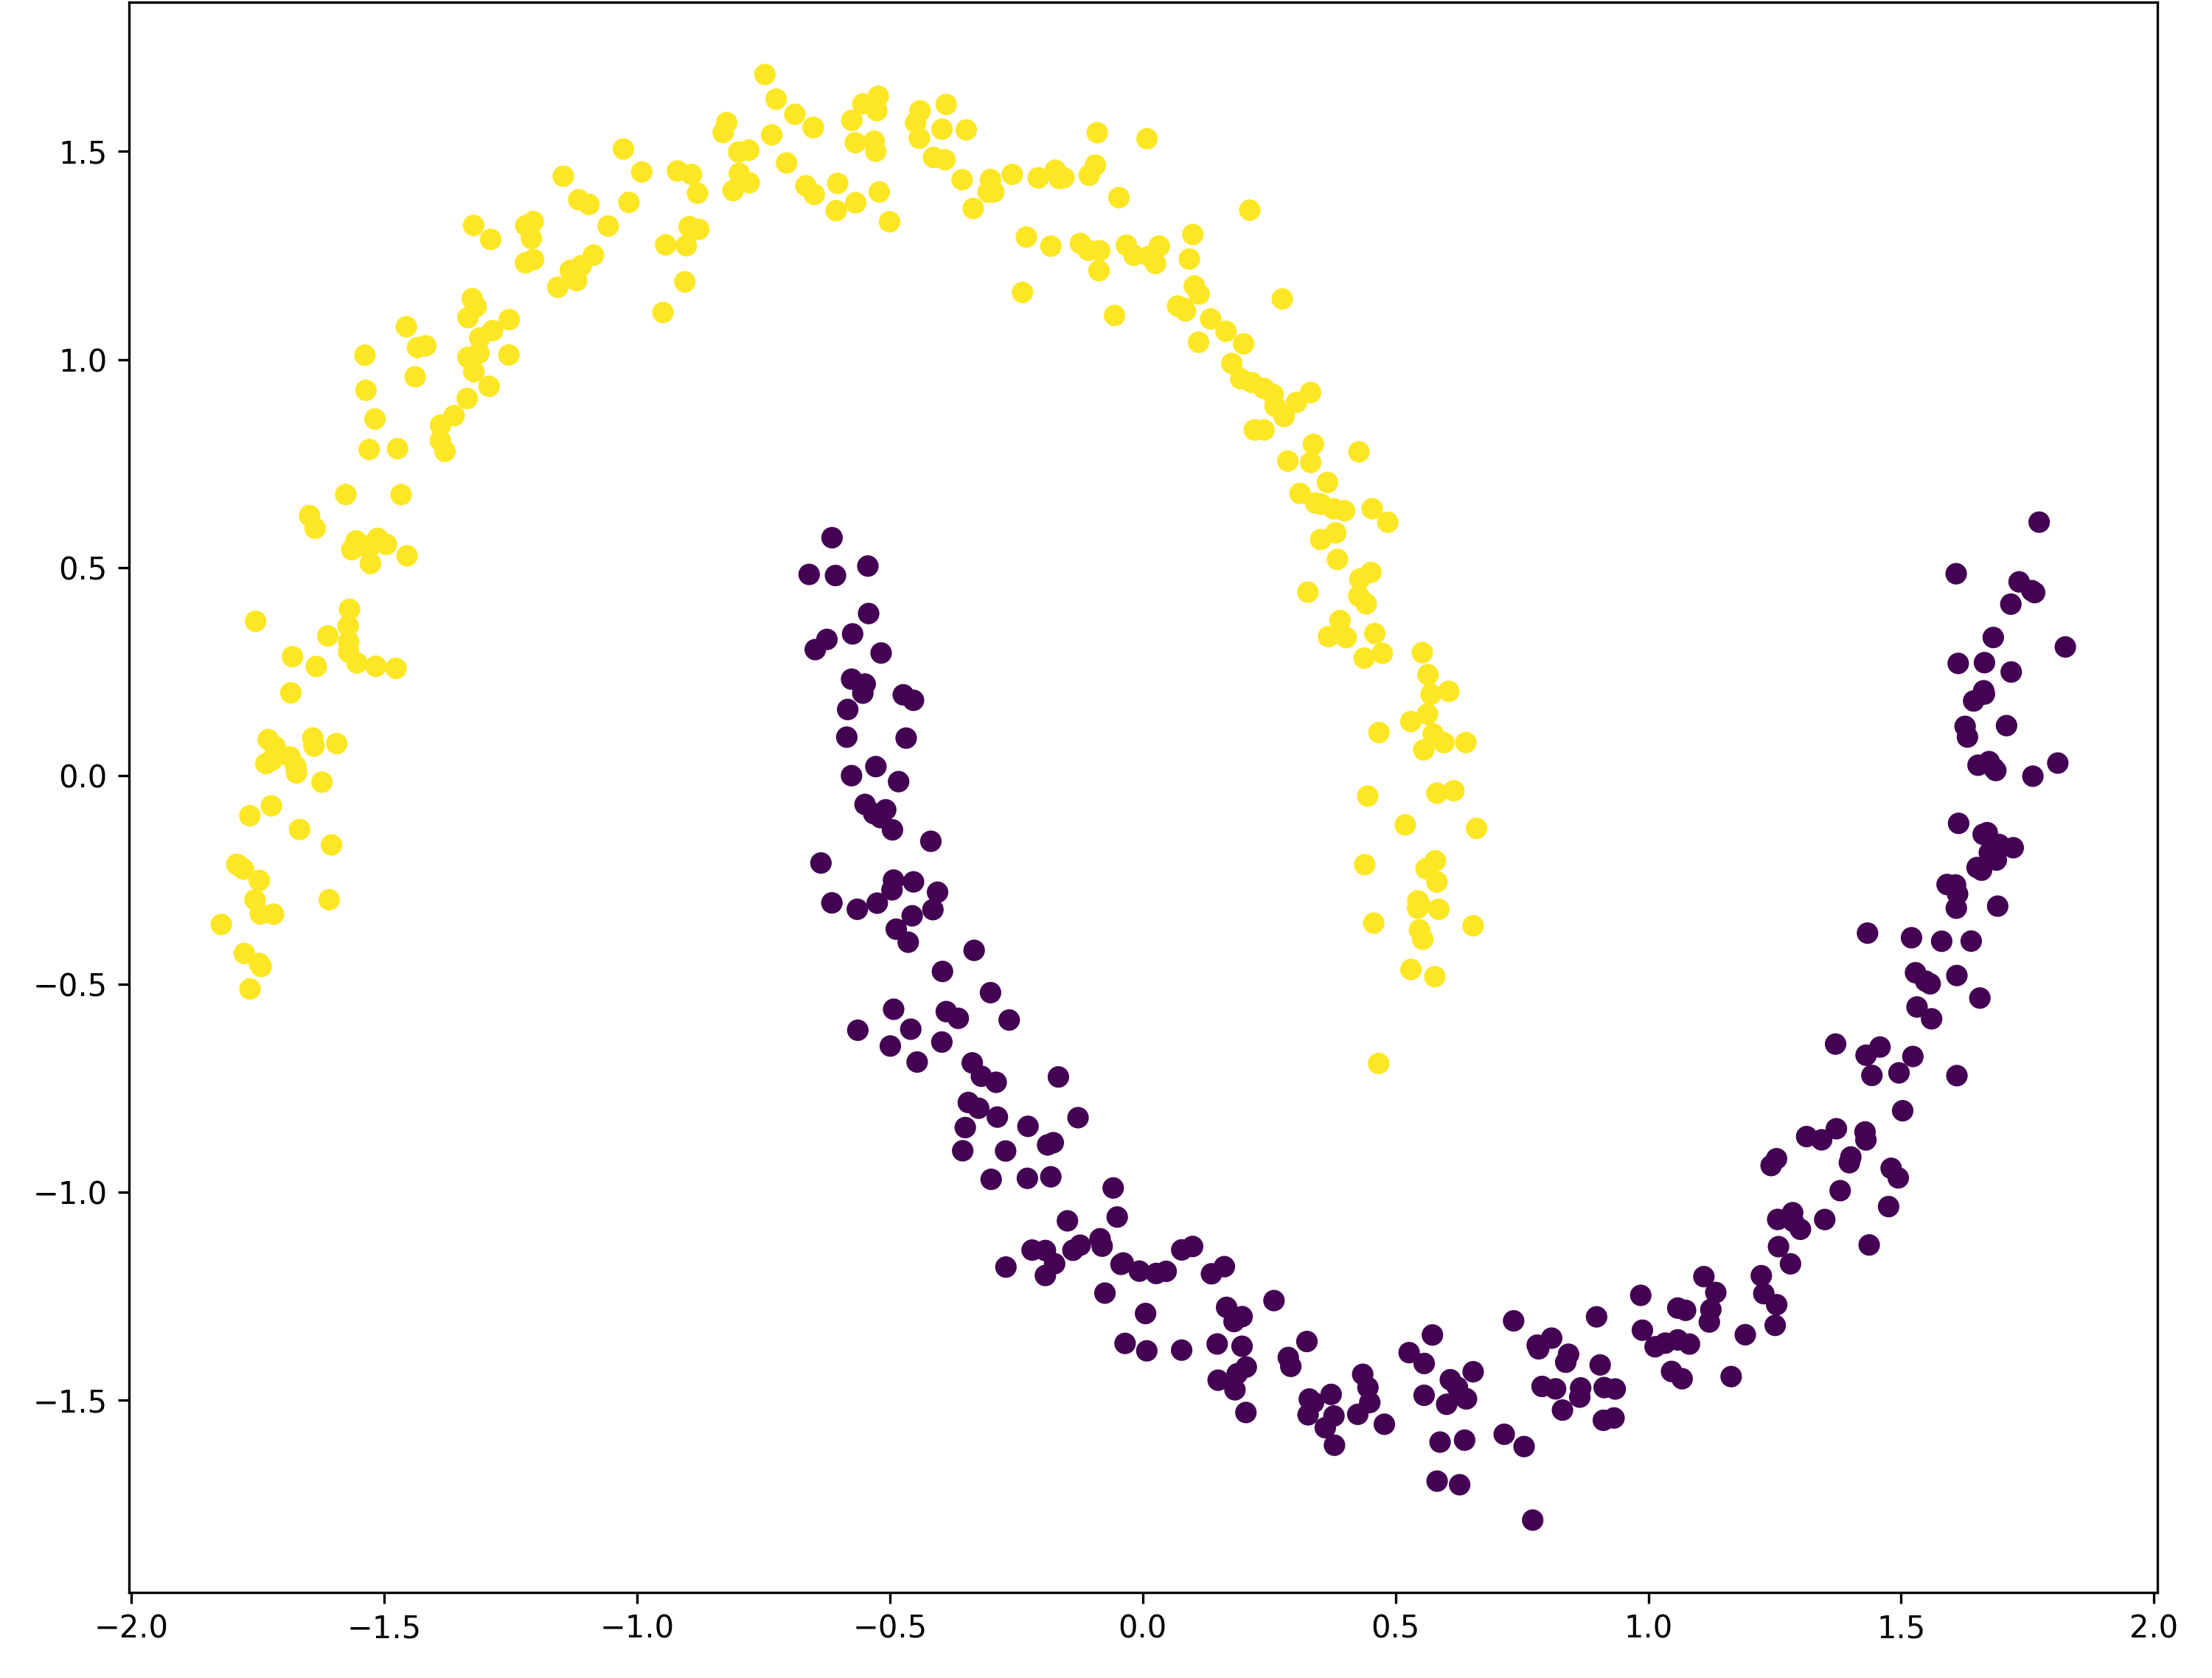
\includegraphics[width=\linewidth]{chapters/fundamentacao/imagens/random_n0_noisy_moons_optics_min_samples_7_xi_0_1_min_cluster_size_0_1.png}
  \subcaption{OPTICS}% (\textsf{xi}$ = 0.1$, \textsf{min\_cluster\_size}$ = 0.1$)}
\end{minipage}%
\hspace{0.02cm}
\begin{minipage}{.35\textwidth}
  \centering
  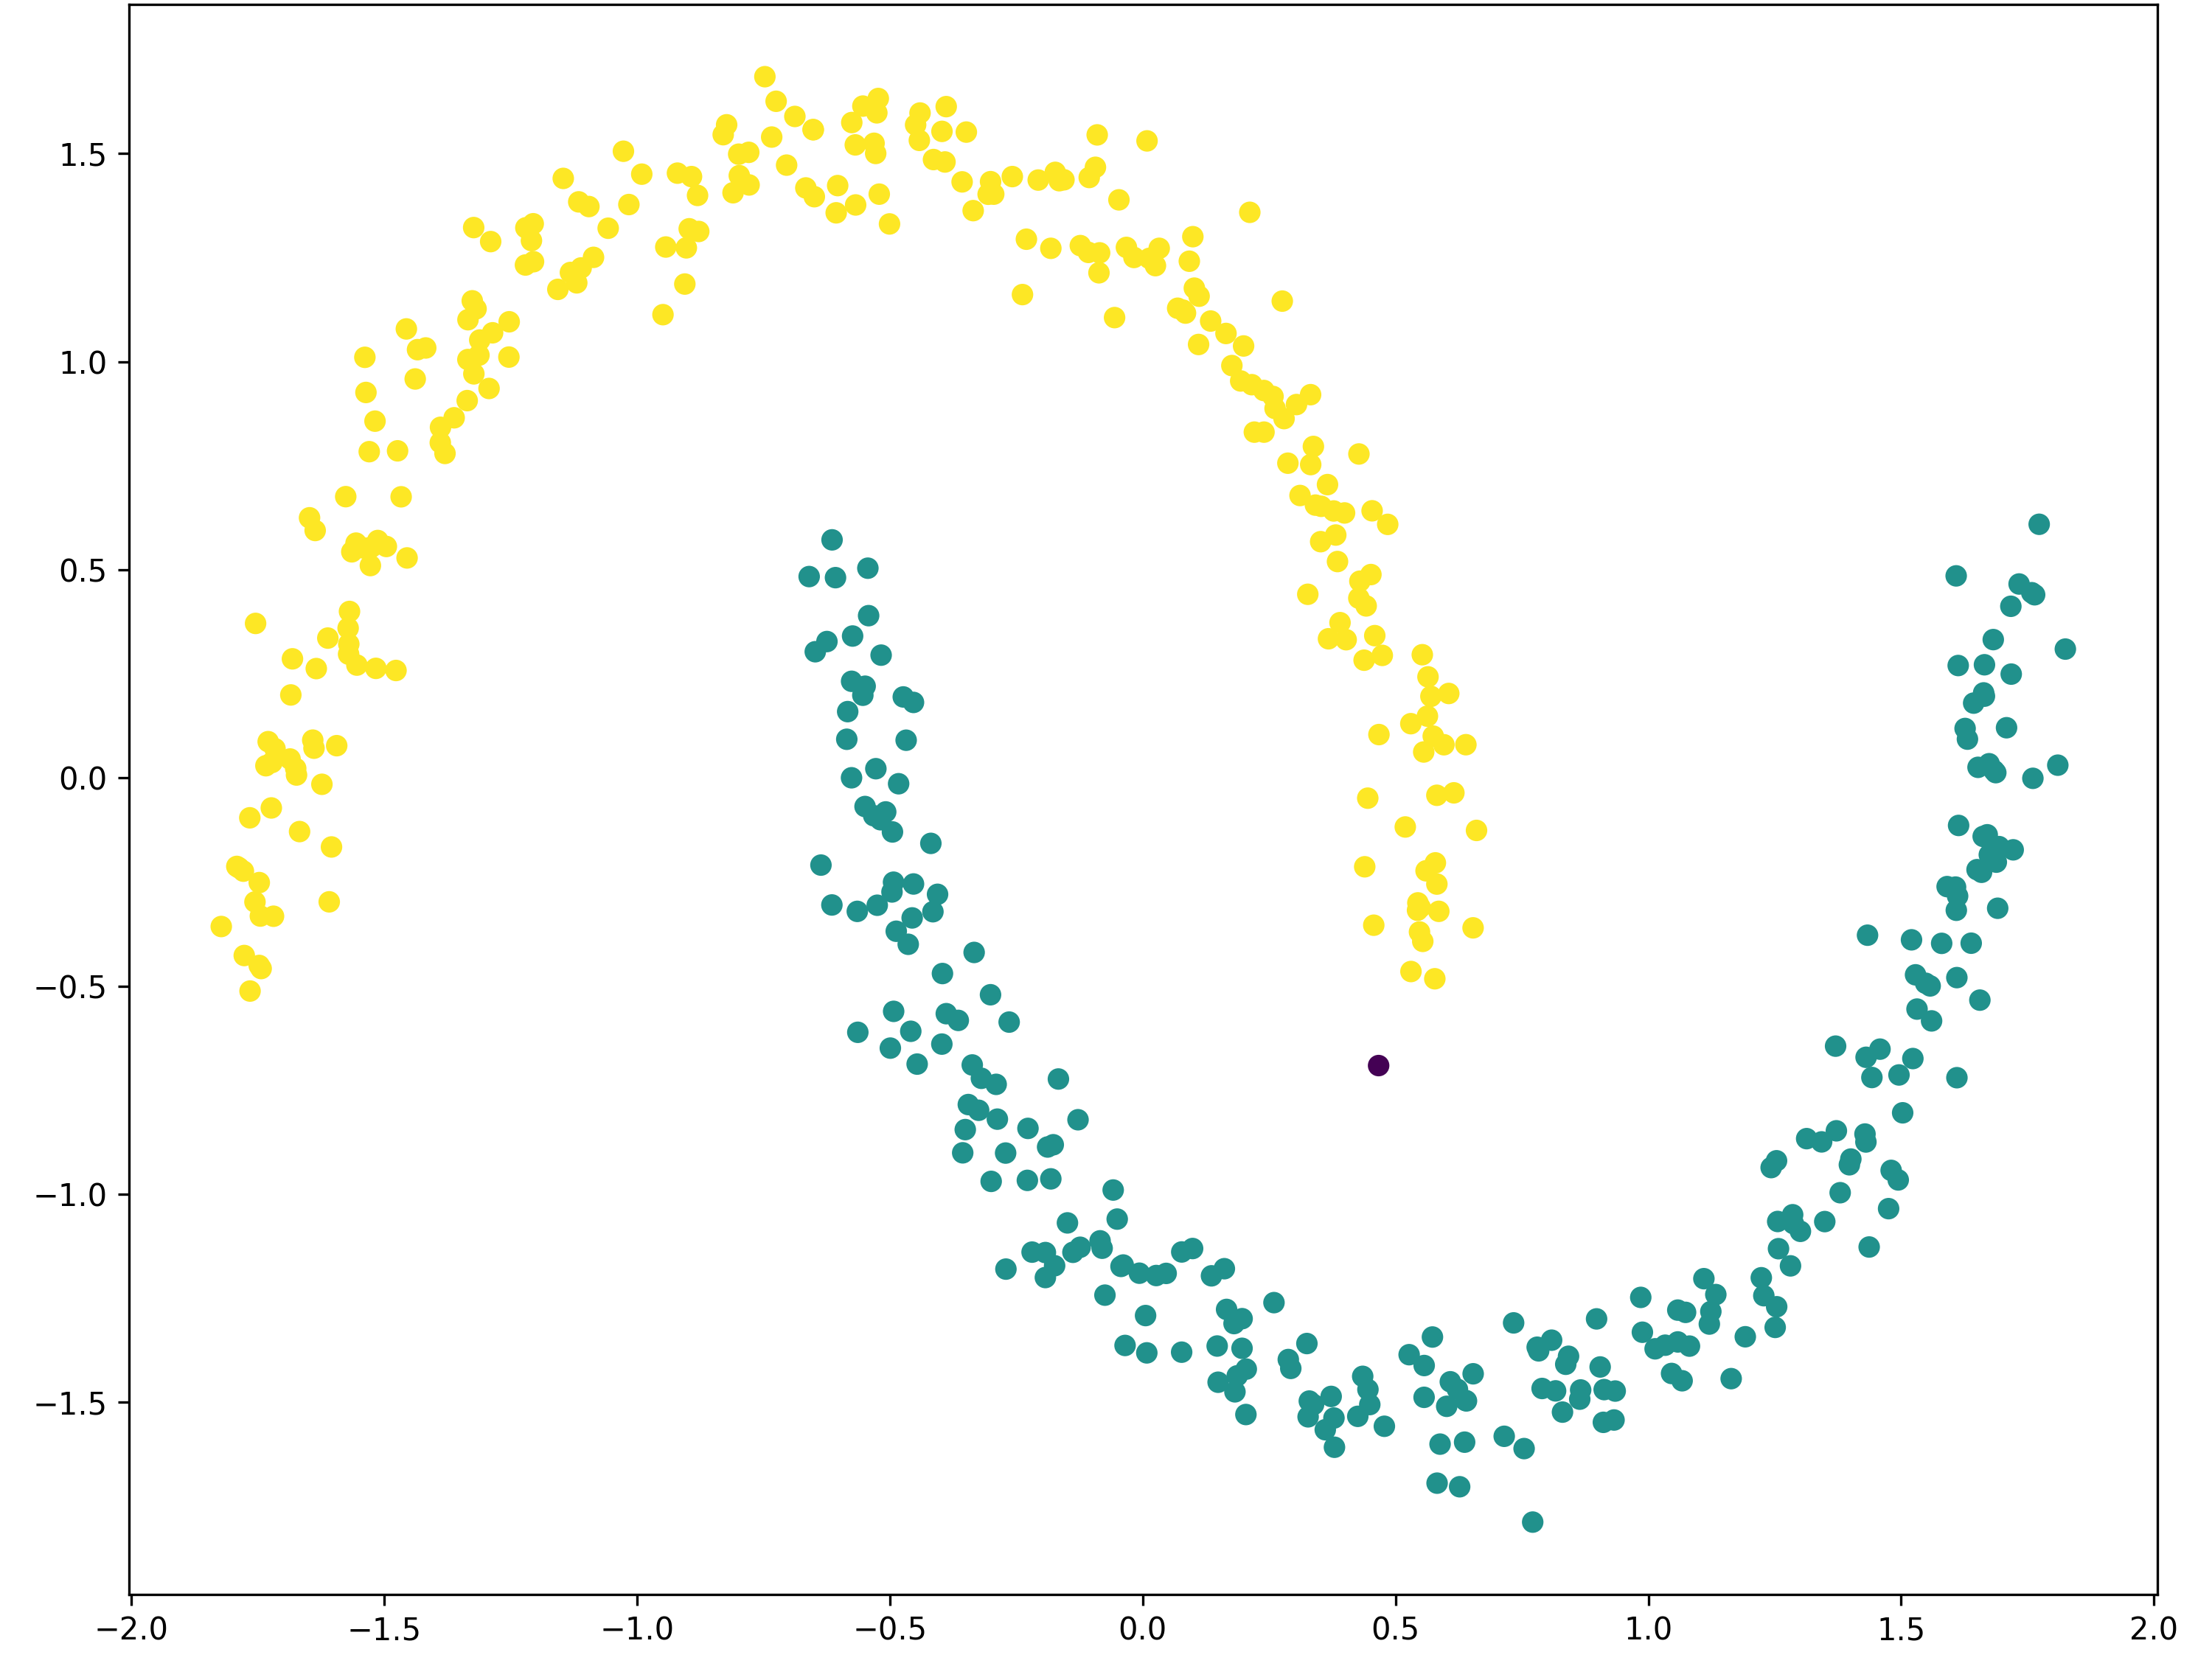
\includegraphics[width=\linewidth]{chapters/fundamentacao/imagens/random_n0_noisy_moons_dbscan_eps_0_2_min_samples_2.png}
  \subcaption{DBSCAN ($\epsilon = 0.2$)}
\end{minipage}
\vspace{0.02cm}
\begin{minipage}{.35\textwidth}
  \centering
  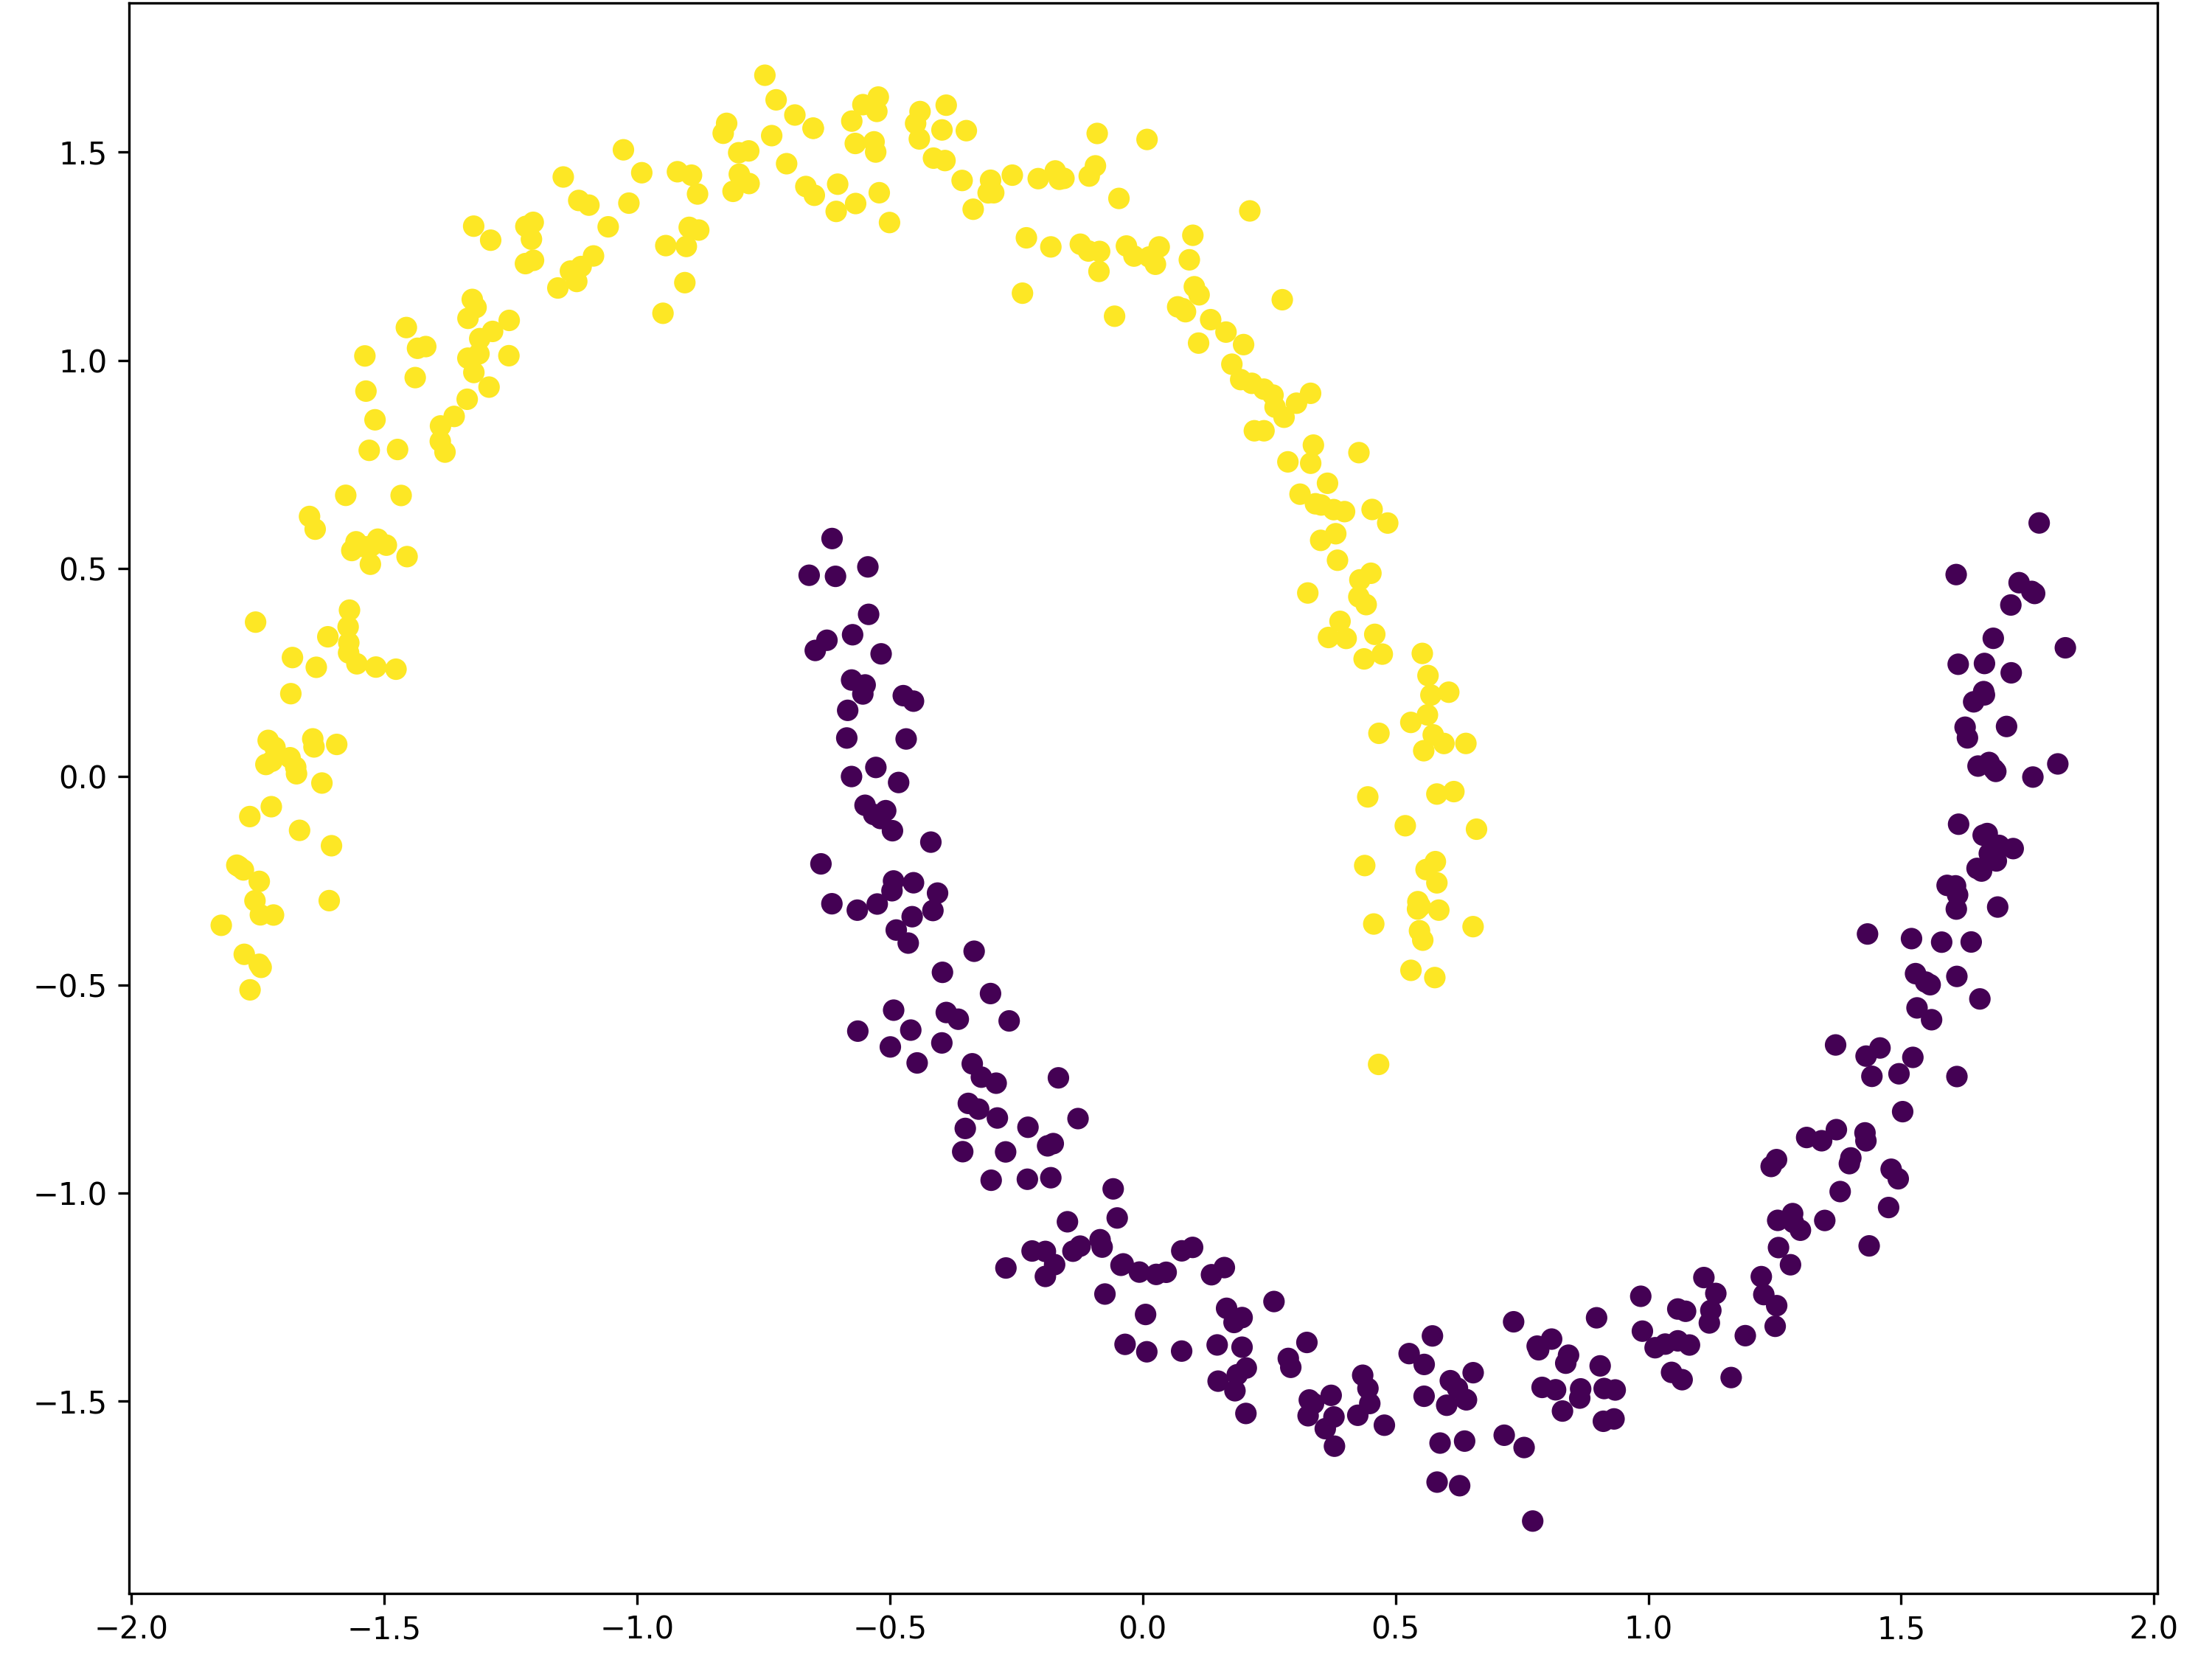
\includegraphics[width=\linewidth]{chapters/fundamentacao/imagens/random_n0_noisy_moons_dbscan_eps_0_3_min_samples_2.png}
  \subcaption{DBSCAN ($\epsilon = 0.3$)}
\end{minipage}%
\hspace{0.02cm}
\begin{minipage}{.35\textwidth}
  \centering
  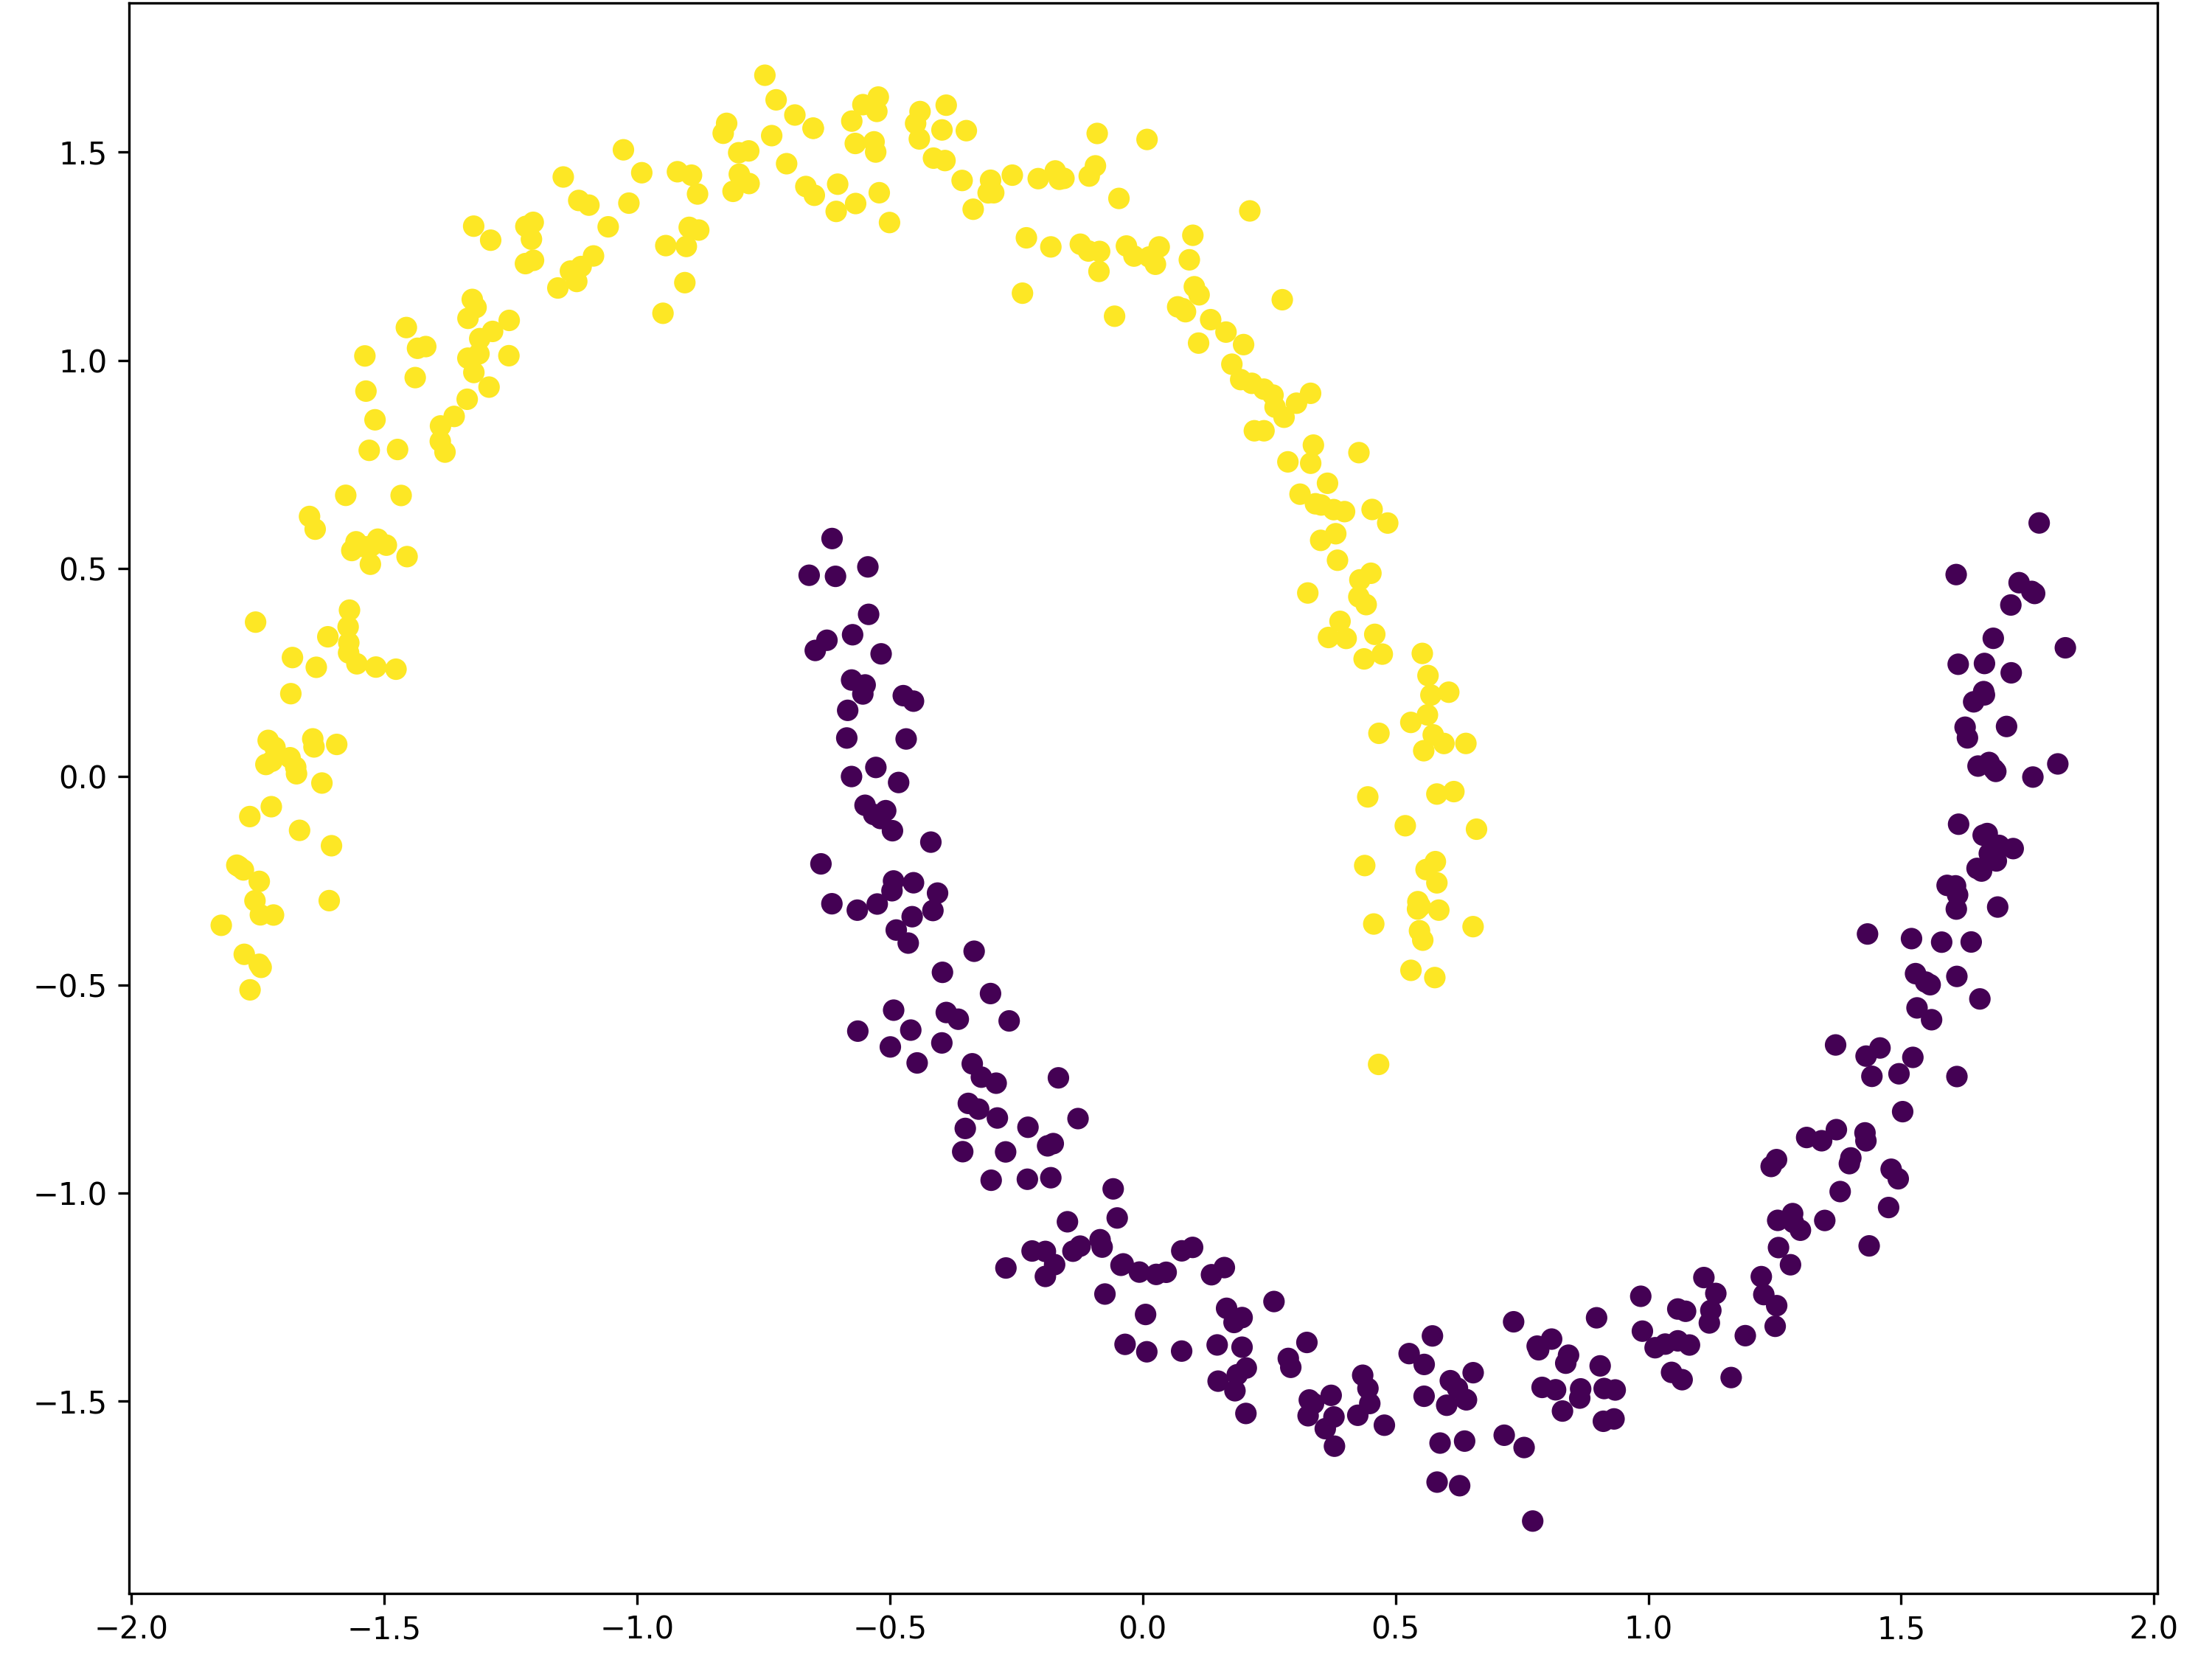
\includegraphics[width=\linewidth]{chapters/fundamentacao/imagens/random_n0_noisy_moons_dbscan_eps_0_4_min_samples_2.png}
  \subcaption{DBSCAN ($\epsilon = 0.4$)}
\end{minipage}

\vspace{0.02cm}
\begin{minipage}{.35\textwidth}
  \centering
  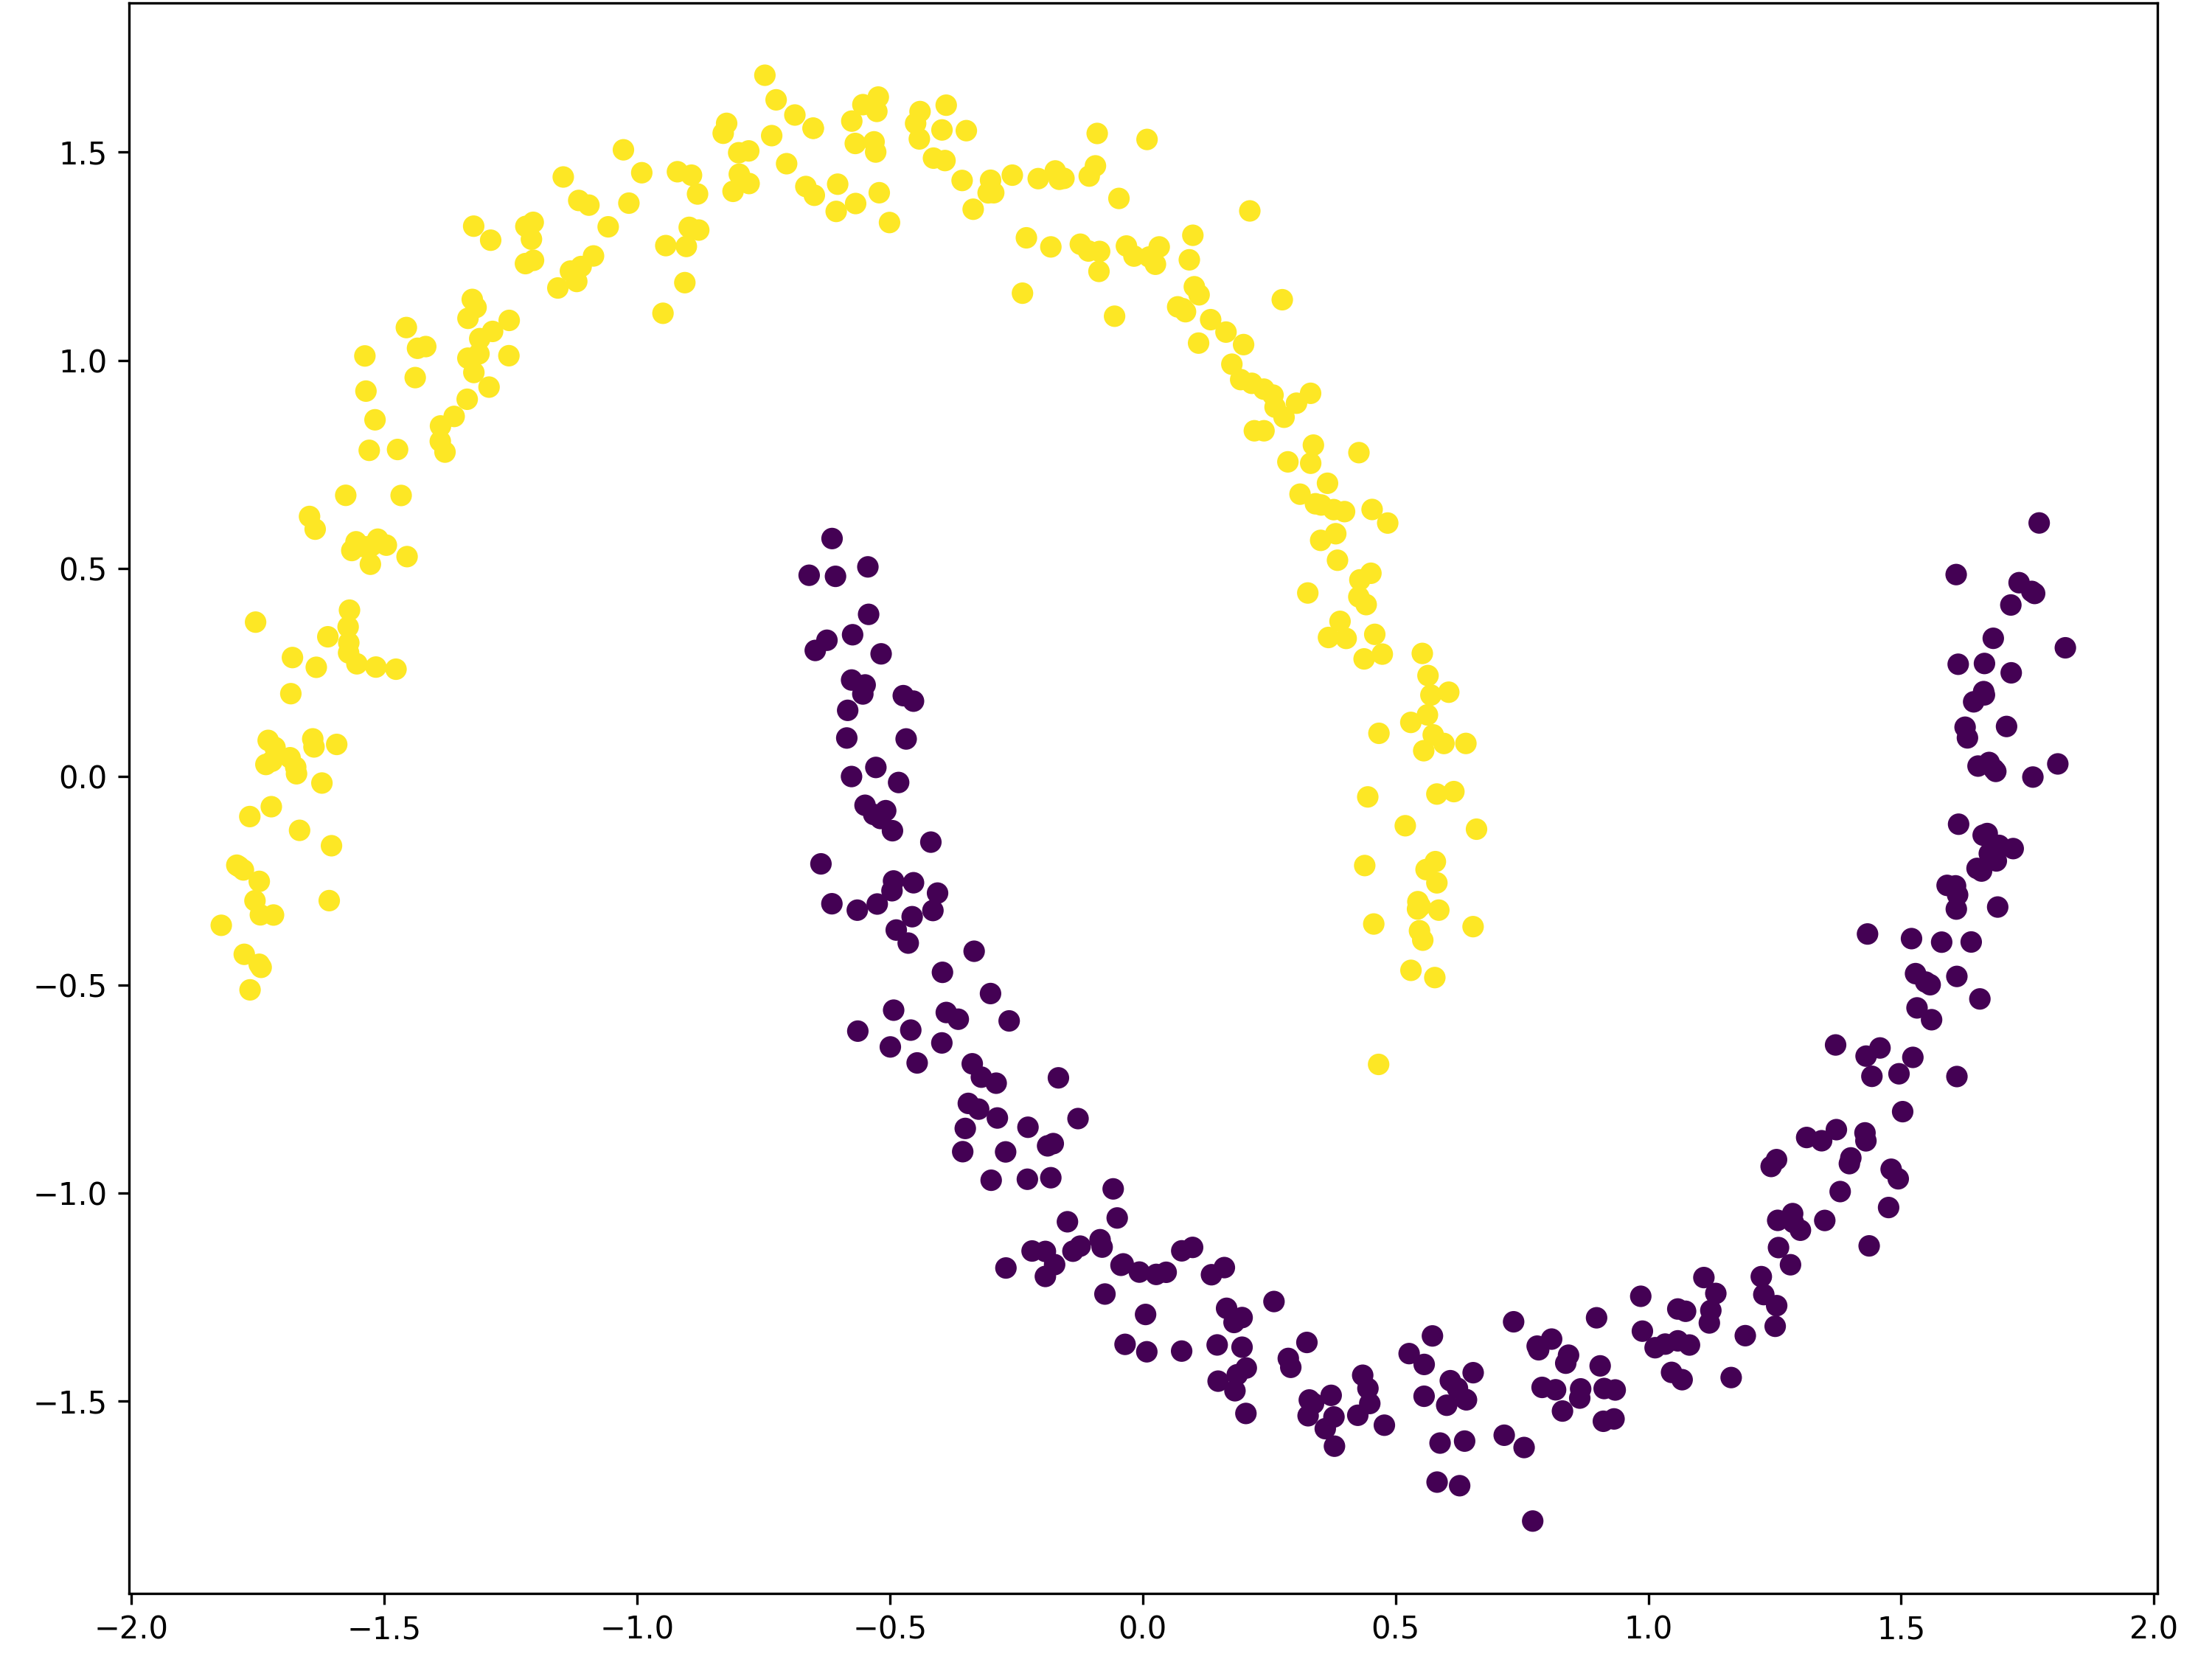
\includegraphics[width=\linewidth]{chapters/fundamentacao/imagens/random_n0_noisy_moons_dbscan_eps_0_5_min_samples_2.png}
  \subcaption{DBSCAN ($\epsilon = 0.5$)}
\end{minipage}%
\hspace{0.02cm}
\begin{minipage}{.35\textwidth}
  \centering
  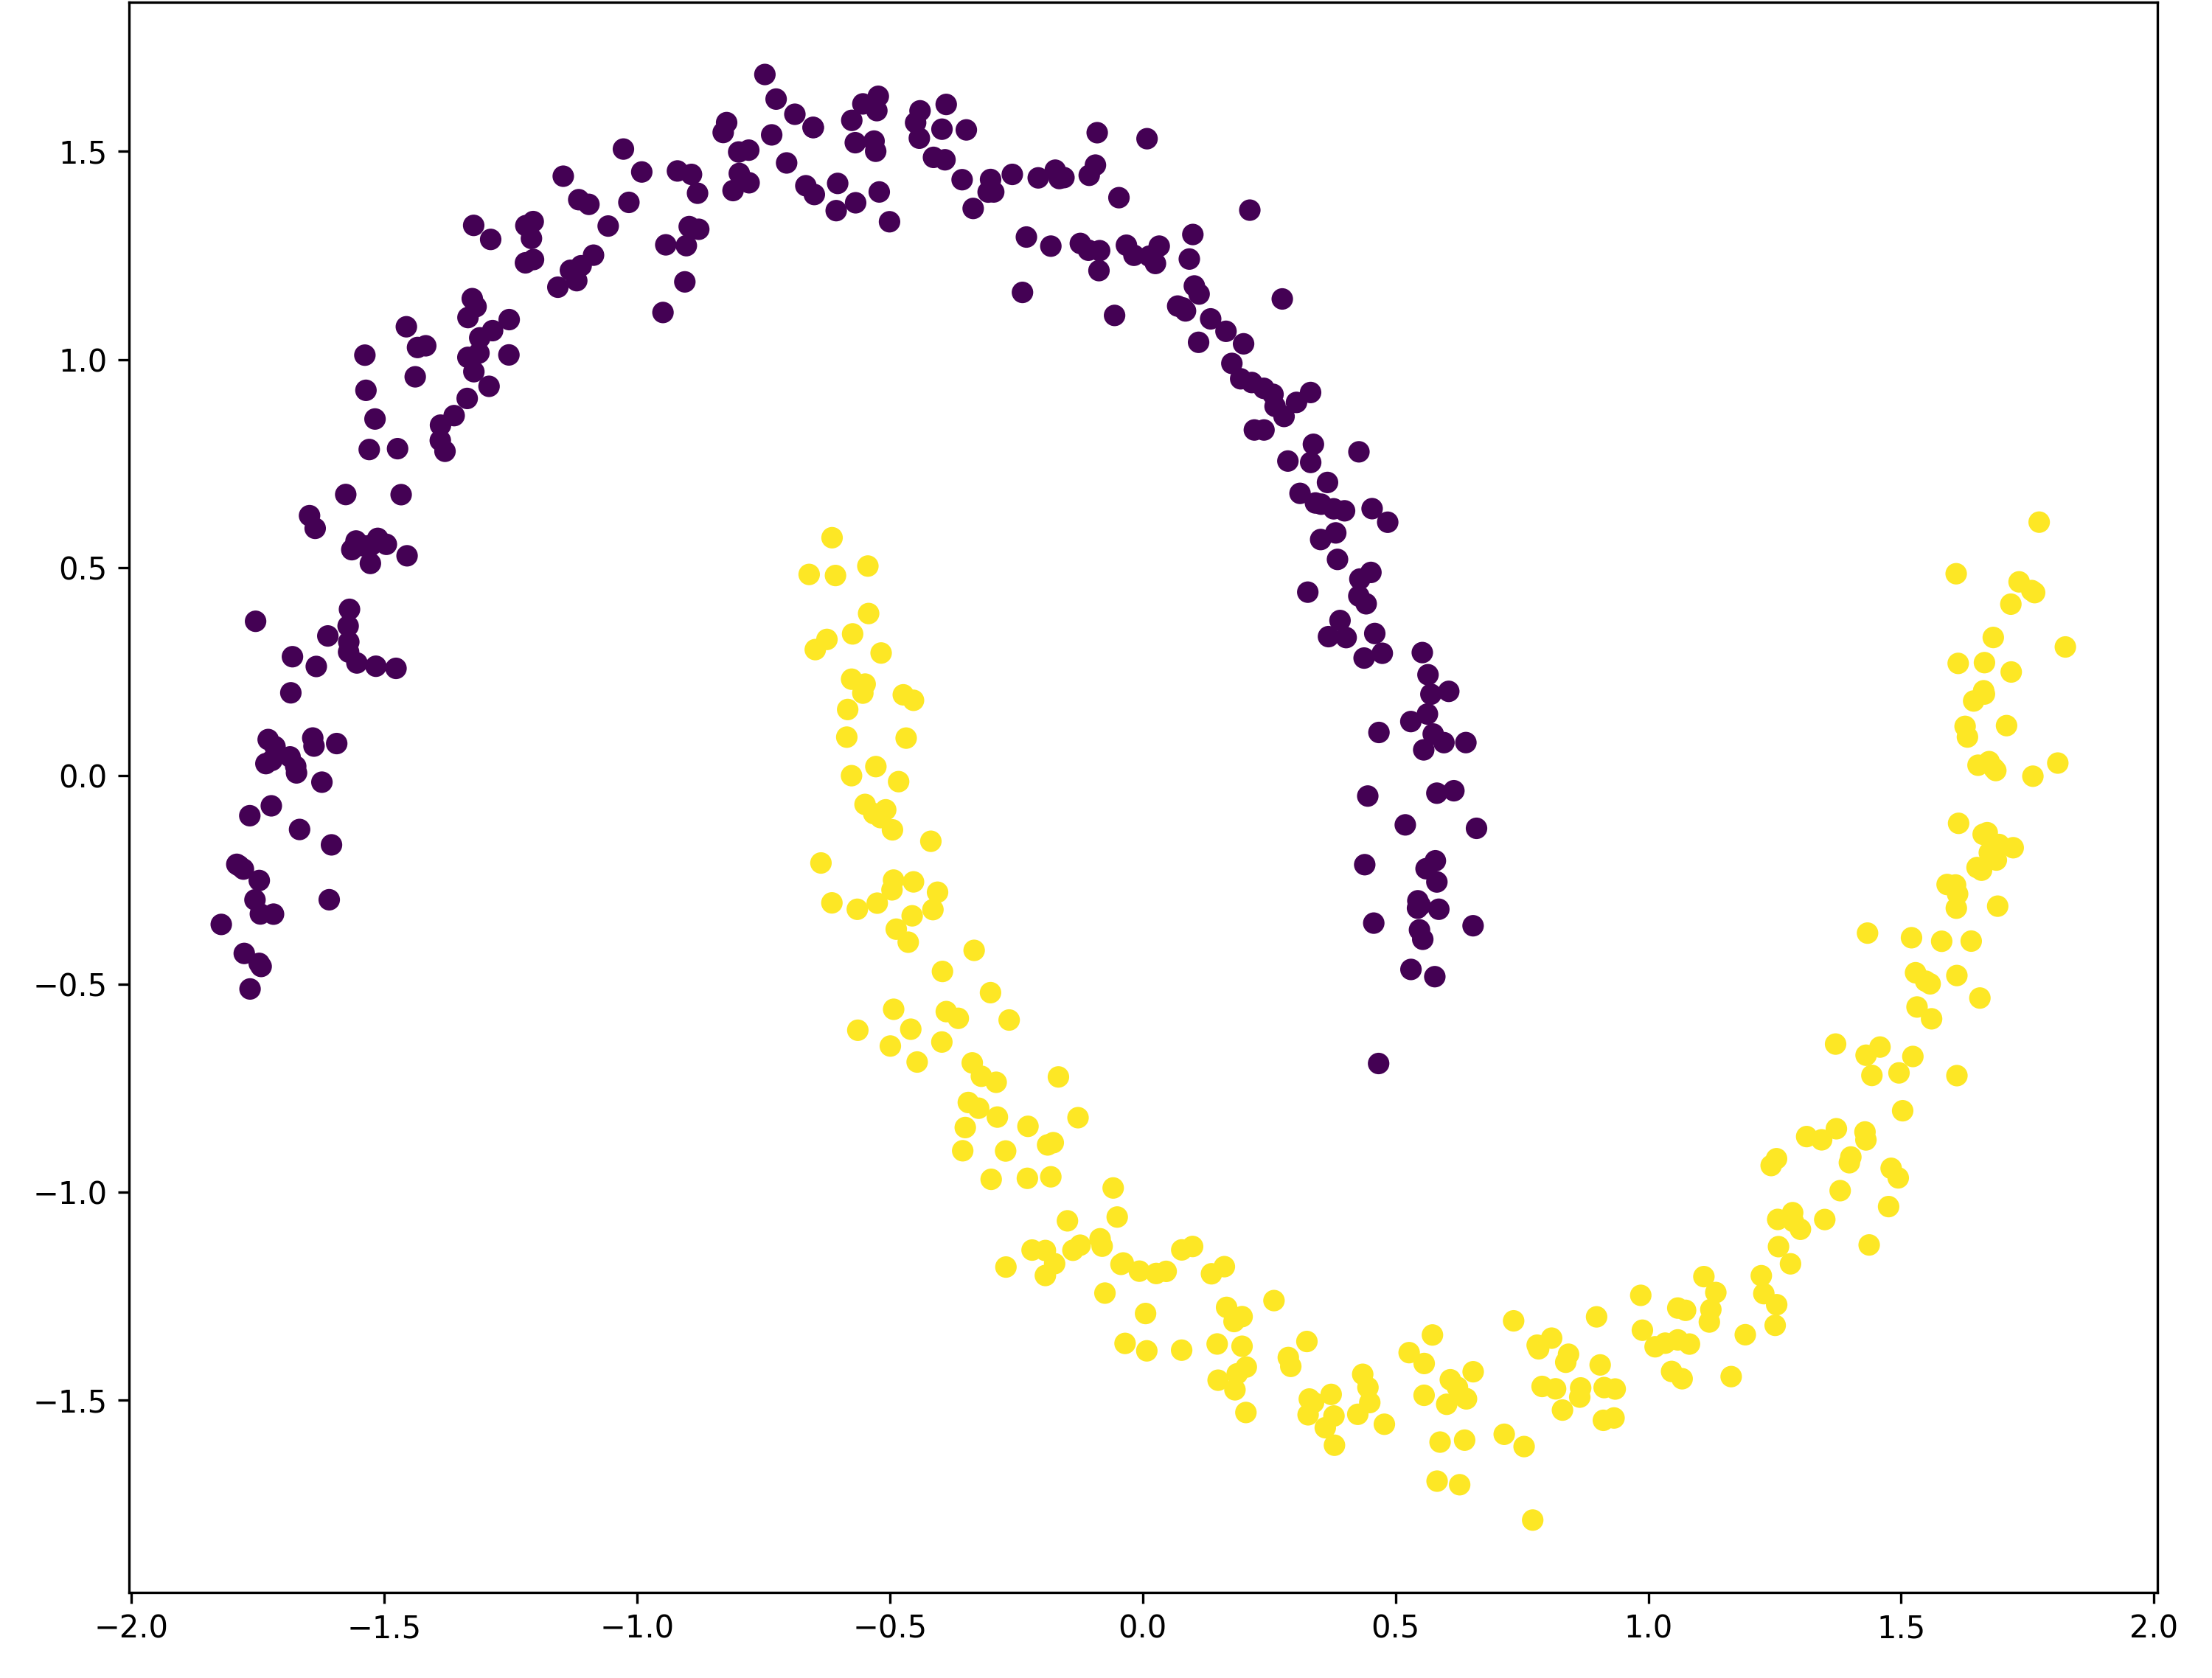
\includegraphics[width=\linewidth]{chapters/fundamentacao/imagens/random_n0_noisy_moons_spectral_clustering_n_clusters_2_eigen_solver_arpack_affinity_nearest_neighbors.png}
  \subcaption{Spectral Clustering ($K = 2$)}
\end{minipage}
\caption{As melhores partições achadas pelo Mean Shift, Spectral Clustering ($K = 2$), DBSCAN ($\epsilon = \{0.2, 0.3, 0.4, 0.5\} $) and OPTICS (\textsf{xi}$ = 0.1$ e
\textsf{min\_cluster\_size}$ = 0.1$), para o conjunto de dados Noisy Moons.}
\label{fig:noisy_moons_dbscan_optics}
\end{figure}


Para o No Structure, modelos com $K = 1$ deveriam ser ranqueados como melhores, contudo, muitos modelos discordaram com  partições com um unico grupo, e de fato, os melhores modelos agruparam os dados com $K = 4$. Acreditamos que isso deve a apenas $3$ dos $37$ modelos ($35$ modelos mais o Average e Best Responses), ajustando explicitamente um unico grupo para o conjunto de dados, tornando mais dificil obter um consenso com sua decisão. Note que a habilidade estimada aparenta estar muito proxima, para todos so conjuntos, porém isso não afeta a capacidade do \gls{CLAIRE} em ranquear os modelos de forma adequada.


\begin{figure}[t]
\centering
\begin{minipage}{.5\textwidth}
  \centering
  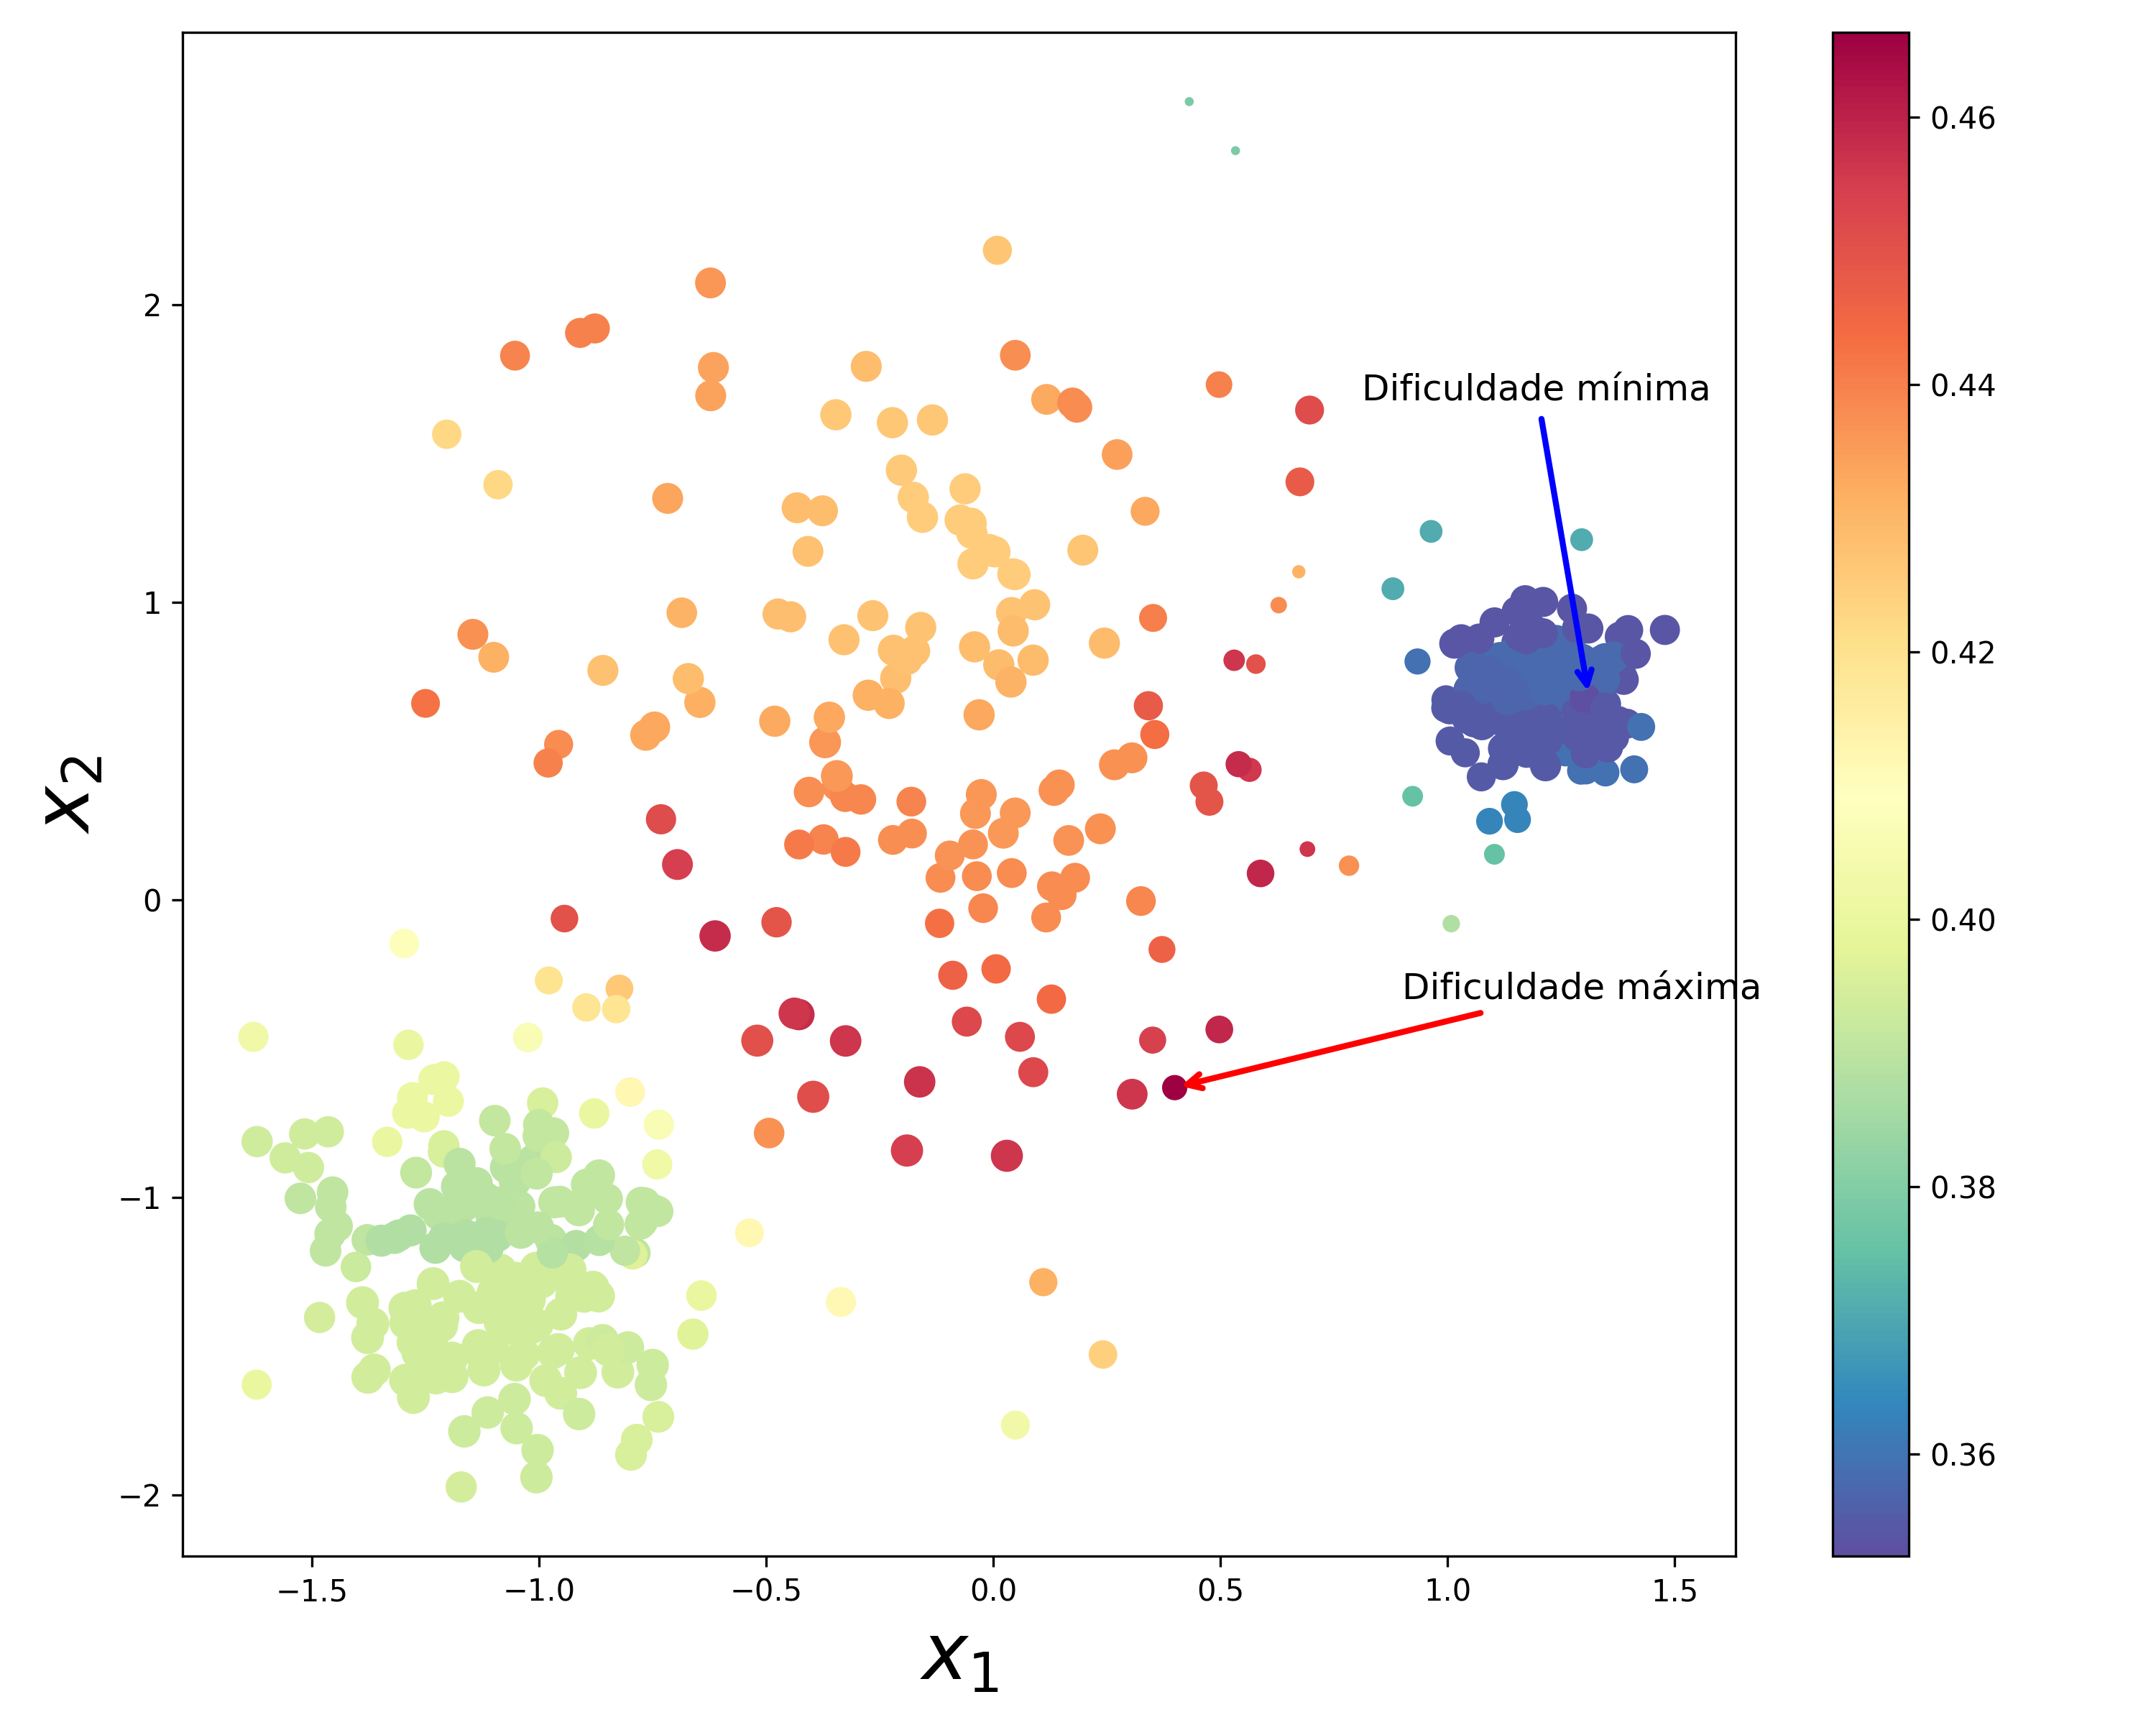
\includegraphics[width=\linewidth]{chapters/fundamentacao/imagens/varied_random_n0_arrow.png}
  % varied_random_n0_difficulties.png
\end{minipage}%
\vspace{.02\textwidth}%
\begin{minipage}{.5\textwidth}
  \centering
  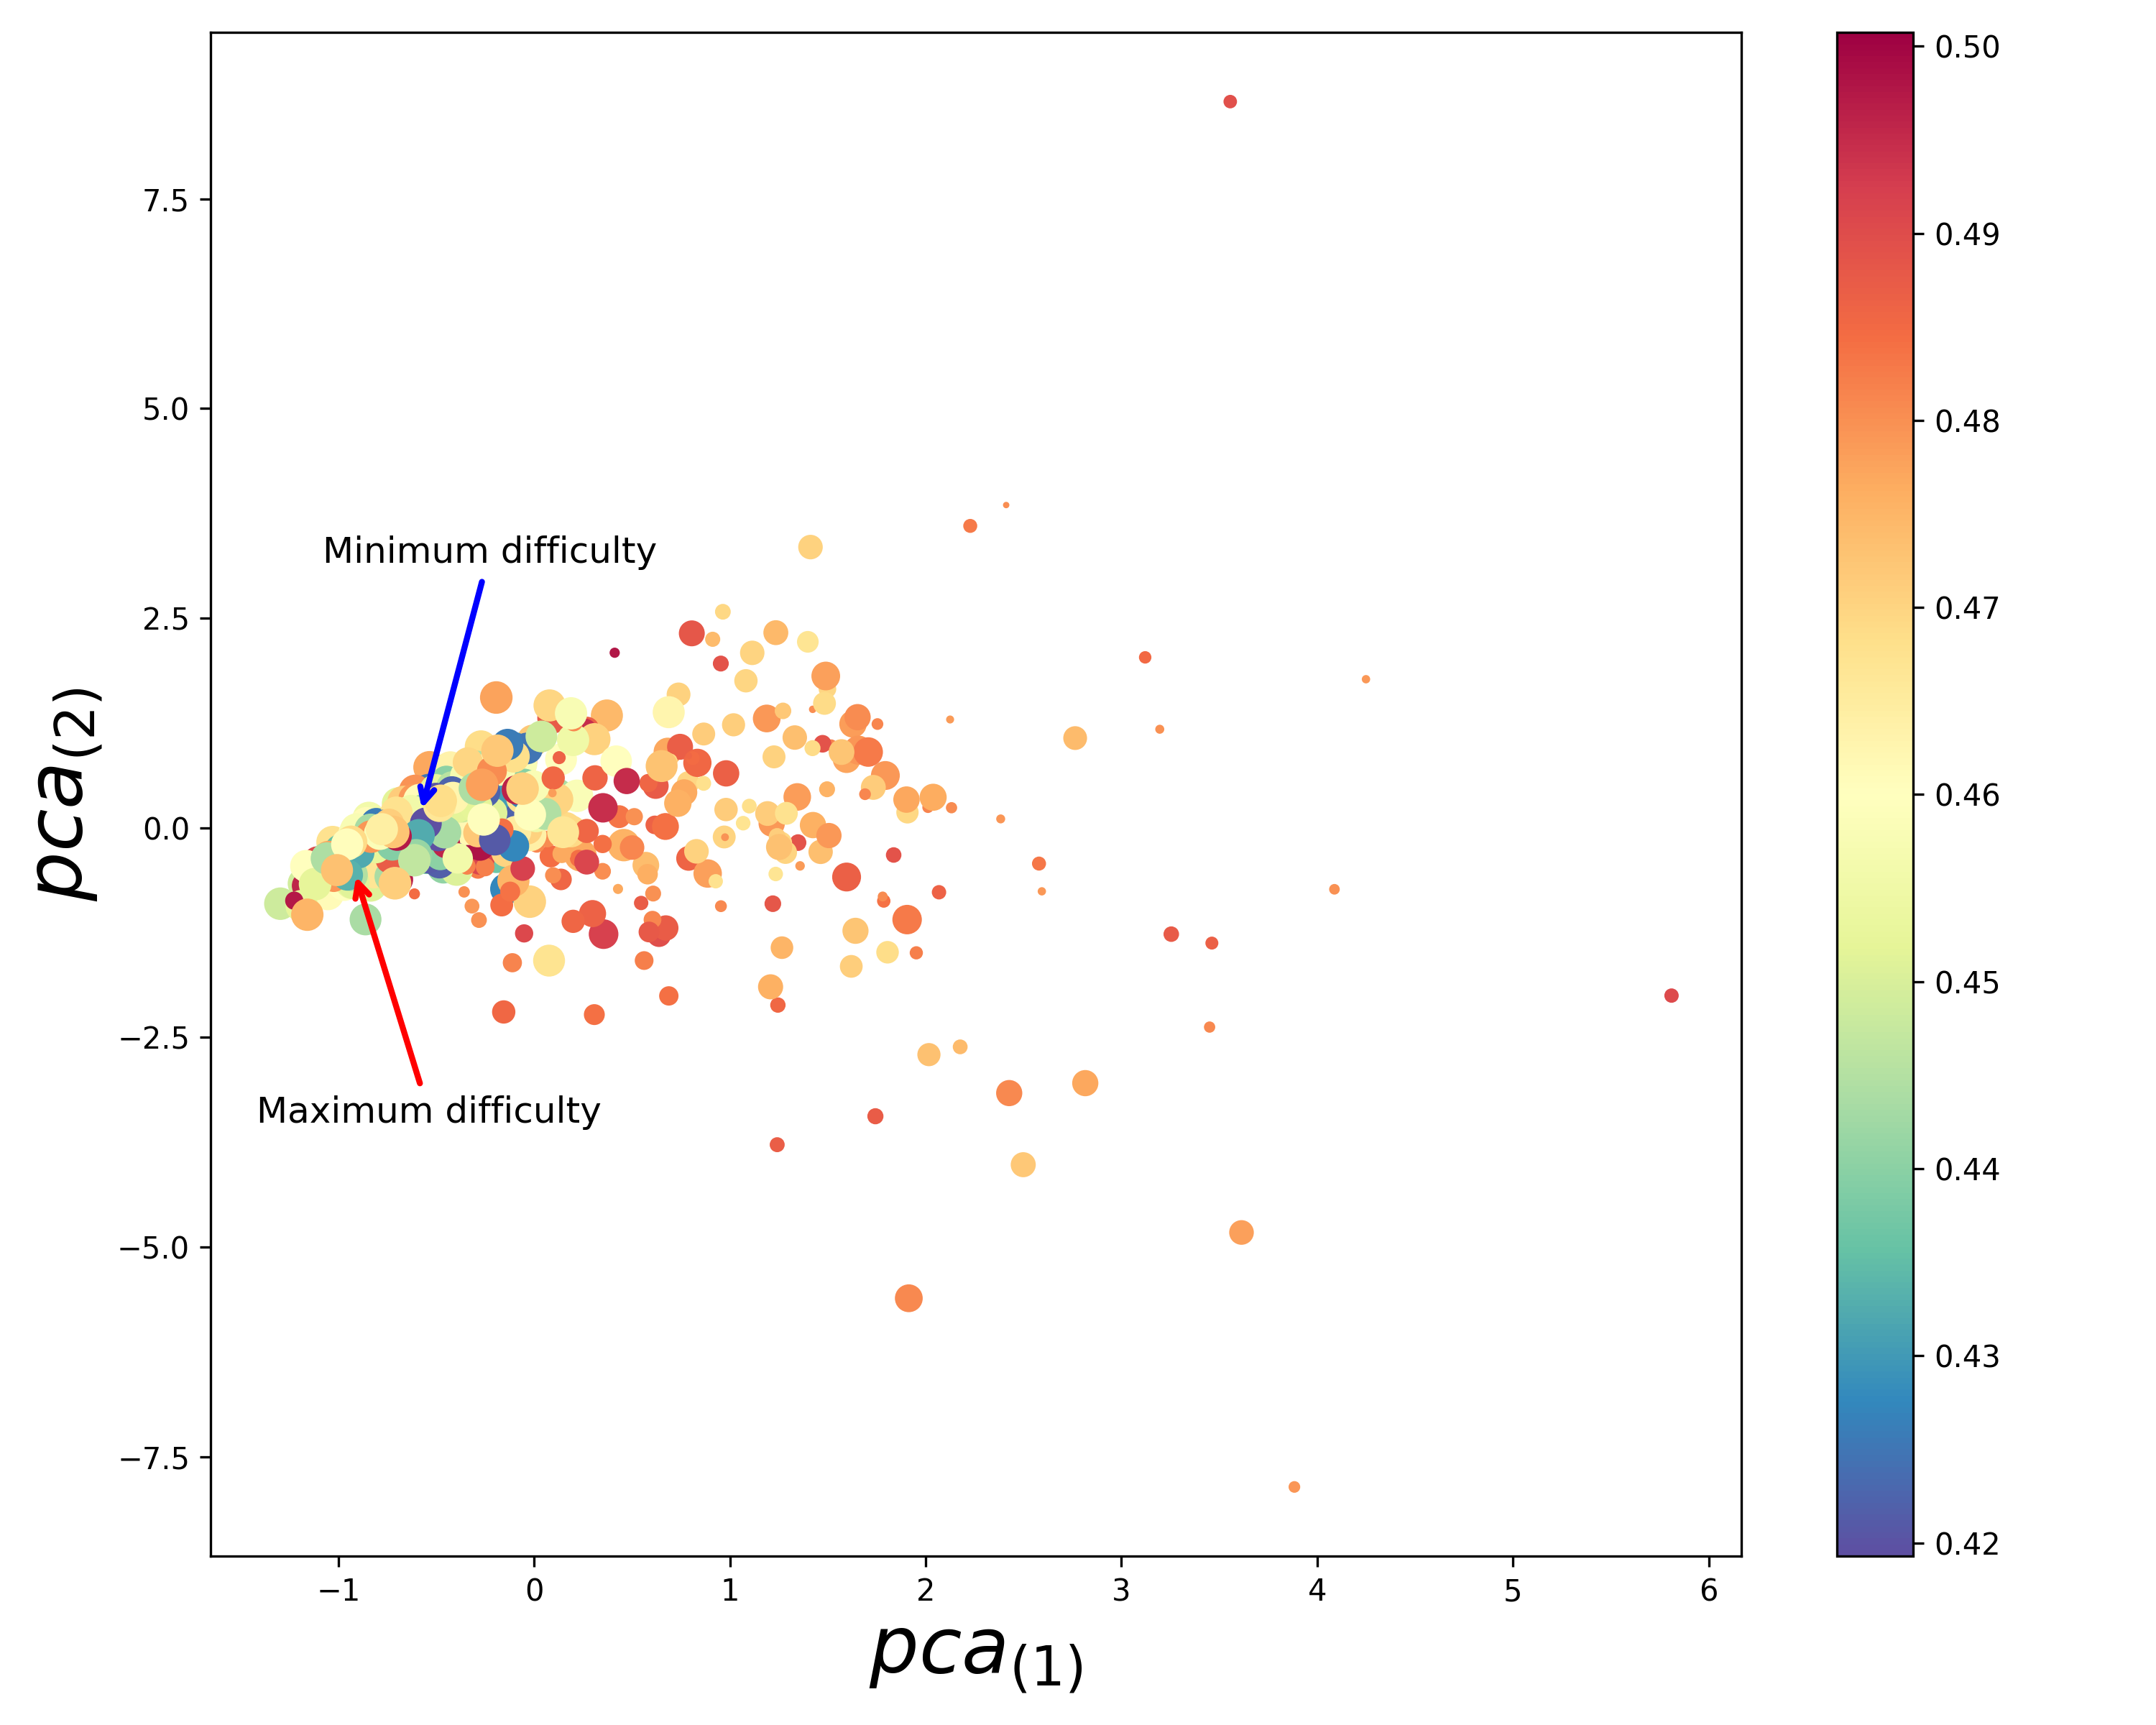
\includegraphics[width=\linewidth]{chapters/fundamentacao/imagens/breast_cancer_random_n0_arrow.png}
  % breast_cancer_random_n0_difficulties.png
\end{minipage}

\caption{Instâncias do conjunto de dados Varied (esquerda) e Breast Cancer (direita), colorido pela dificuldade e com os pontos com tamanho correspondente ao discriminante. Setas  azul e vermelhas indicam as instâncias mais faceis e mais dificeis, respectivamente, para cada conjunto de dados.}
\label{fig:combined_figures_diff_disc}
\end{figure}


Como mencionado nos parágrafos anteriores, uma das vantagens do \gls{CLAIRE} sobre outros meios de ranqueamento de modelos de agrupamento, é que ele é capaz de proporcionar uma avaliação das instâncias de um conjunto de dados, por meio das dificuldades e discriminantes estimados, além de trazer uma camada maior de robustez à estimação da habilidade. Como podemos ver na figura \ref{fig:combined_figures_diff_disc}, aonde certas áreas do espaço de variáveis (ilustrado por tons mais escuros de vermelho) tendem a conter instâncias que os modelos possuem uma dificuldade maior em concordar. Essas instâncias dessa região possuem altas dificuldades estimadas e são frequentemente  alocadas em regiões de fronteiras, como visto pelo conjutno de dados Varied. Analisando o espaço obtido pelo PCA para o conjunto de dados Breast Cancer, é possivel ver que modelos tendem a discordar muito quando as instâncias pertencem ao cluster mais a direita, porém para o cluster a esquerda possui instâncias mais faceis.

A Figura \ref{fig:easy:hard:clas} apresenta as \gls{CCI}s das instâncias mais fácil e mais difícil do conjunto Varied. No caso da instância mais fácil (Figura \ref{fig:easy_dataset}), qualquer modelo com habilidade superior a $0.35$, ou seja, todos os modelos do nosso conjunto para esse dataset, como visto na tabela \ref{tab:abilities_aniso_blobs_varied_moons_circles_no_structure}, possui resposta esperada (nível de concordância) acima de $0.5$. Observa-se que essa instância está situada no interior de um cluster bem definido, como indicado pela seta azul na Figura \ref{fig:combined_figures_diff_disc}, o que naturalmente favorece elevada concordância entre os modelos. Por outro lado, na instância mais difícil (Figura \ref{fig:hard_class_dataset}), apenas modelos com habilidade superior a $0.47$ apresentam resposta esperada acima de $0.5$, sendo que uma parcela considerável do conjunto (incluindo o OPTICS, a maioria das versões do DBSCAN, K-means e Kernel K-means com $K=1$, além de diversas configurações de Spectral Clustering) apresenta baixo desempenho nesse caso. Essa instância encontra-se na borda do cluster central, maior e mais disperso (ver seta vermelha na Figura \ref{fig:combined_figures_diff_disc}), de modo que alguns modelos a agrupam no cluster central, versões do DBSCAN a classificam como ruído, e métodos que identificam diferentes números de clusters a alocam de maneiras distintas, resultando em baixa concordância.

Discriminações mais elevadas, representadas por pontos maiores na Figura \ref{fig:combined_figures_diff_disc}, tendem a concentrar-se em regiões mais fáceis, pois são essas instâncias que frequentemnete diferenciam modelos mais fortes dos mais fracos. Esse comportamento foi observado no conjunto Varied e também relatado em aplicações anteriores da \gls{TRI} em \gls{AM} \cite{chen2019birt,moraes2020item,moraes2022evaluating}, nas quais itens mais fáceis apresentaram maior discriminação. Entretanto, no conjunto Breast Cancer, diversas instâncias difíceis localizadas à direita também se mostraram altamente discriminativas, indicando que apenas os modelos mais capazes conseguiram agrupá-las corretamente. Esse resultado possui implicações relevantes para reconhecimento de padrões, já que instâncias simultaneamente difíceis e discriminativas podem ser candidatas promissoras para análises mais aprofundadas e melhor compreensão da tarefa.

\begin{figure}[t]%htbp]
    \centering    
    \begin{minipage}[b]{0.47\linewidth}
        \centering
        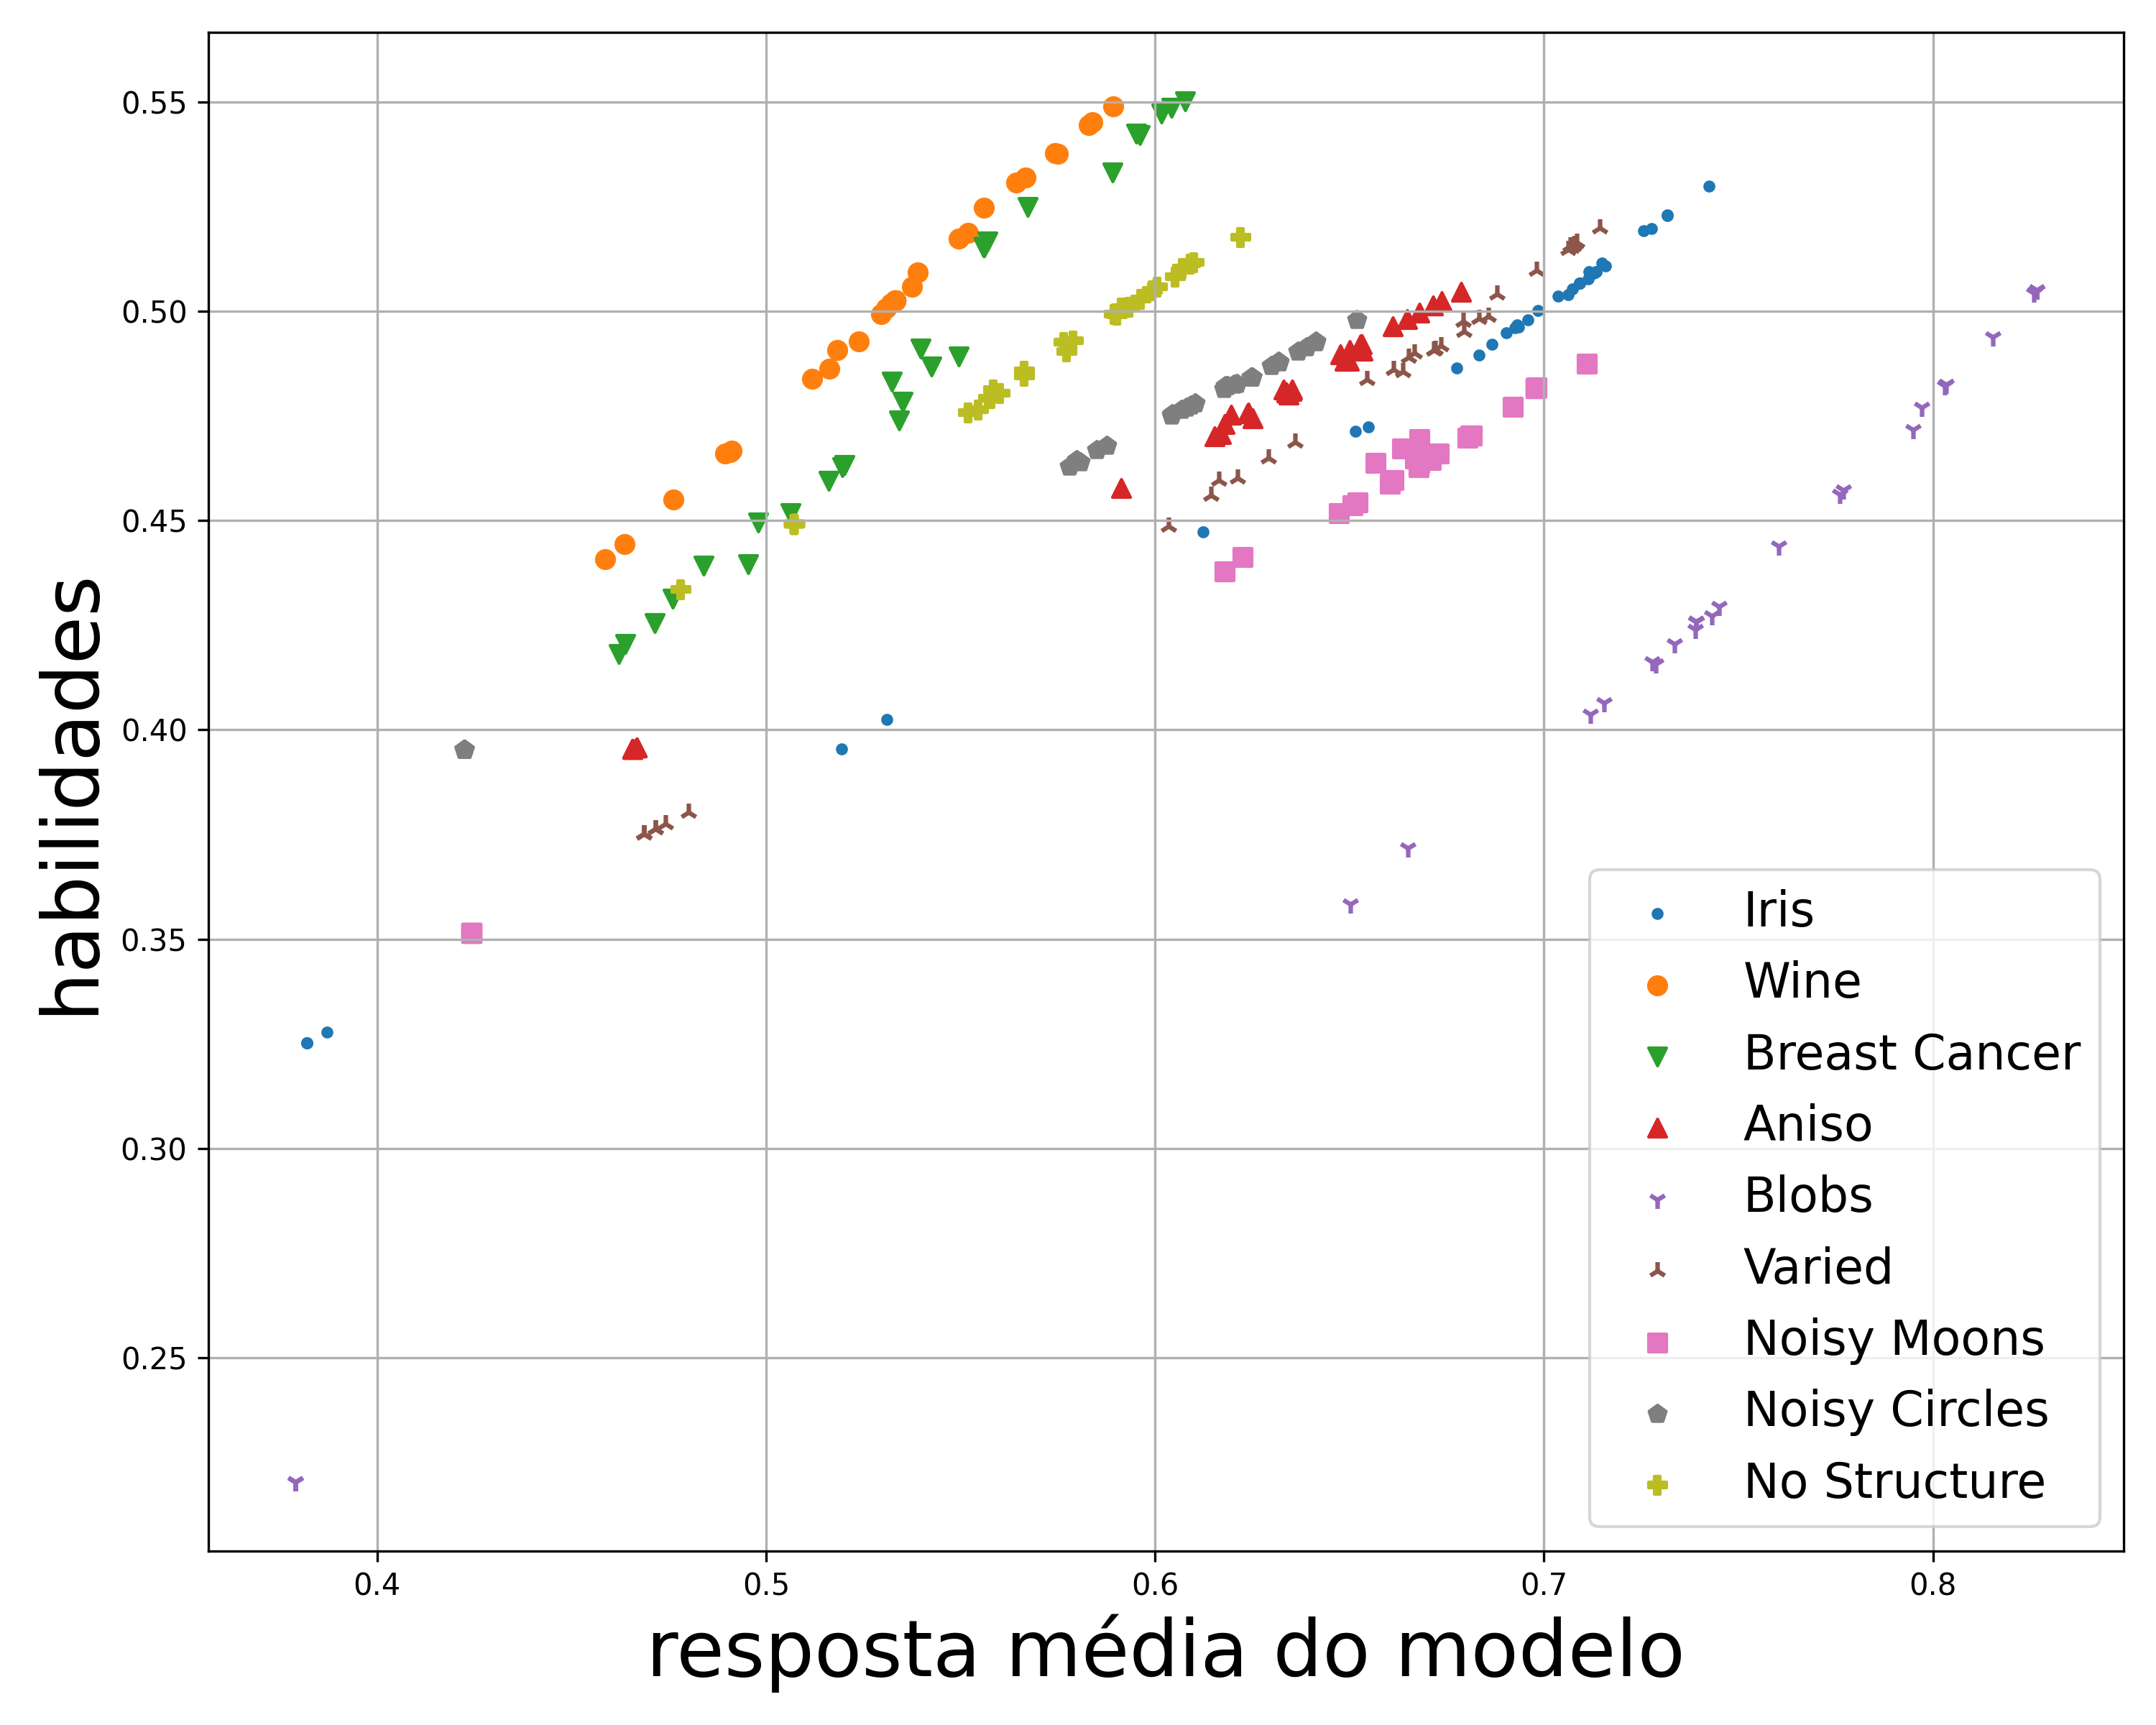
\includegraphics[width=\linewidth]{chapters/fundamentacao/imagens/random_n0_abi_versus_all.png}
    \end{minipage}
    \begin{minipage}[b]{0.47\linewidth}
        \centering
        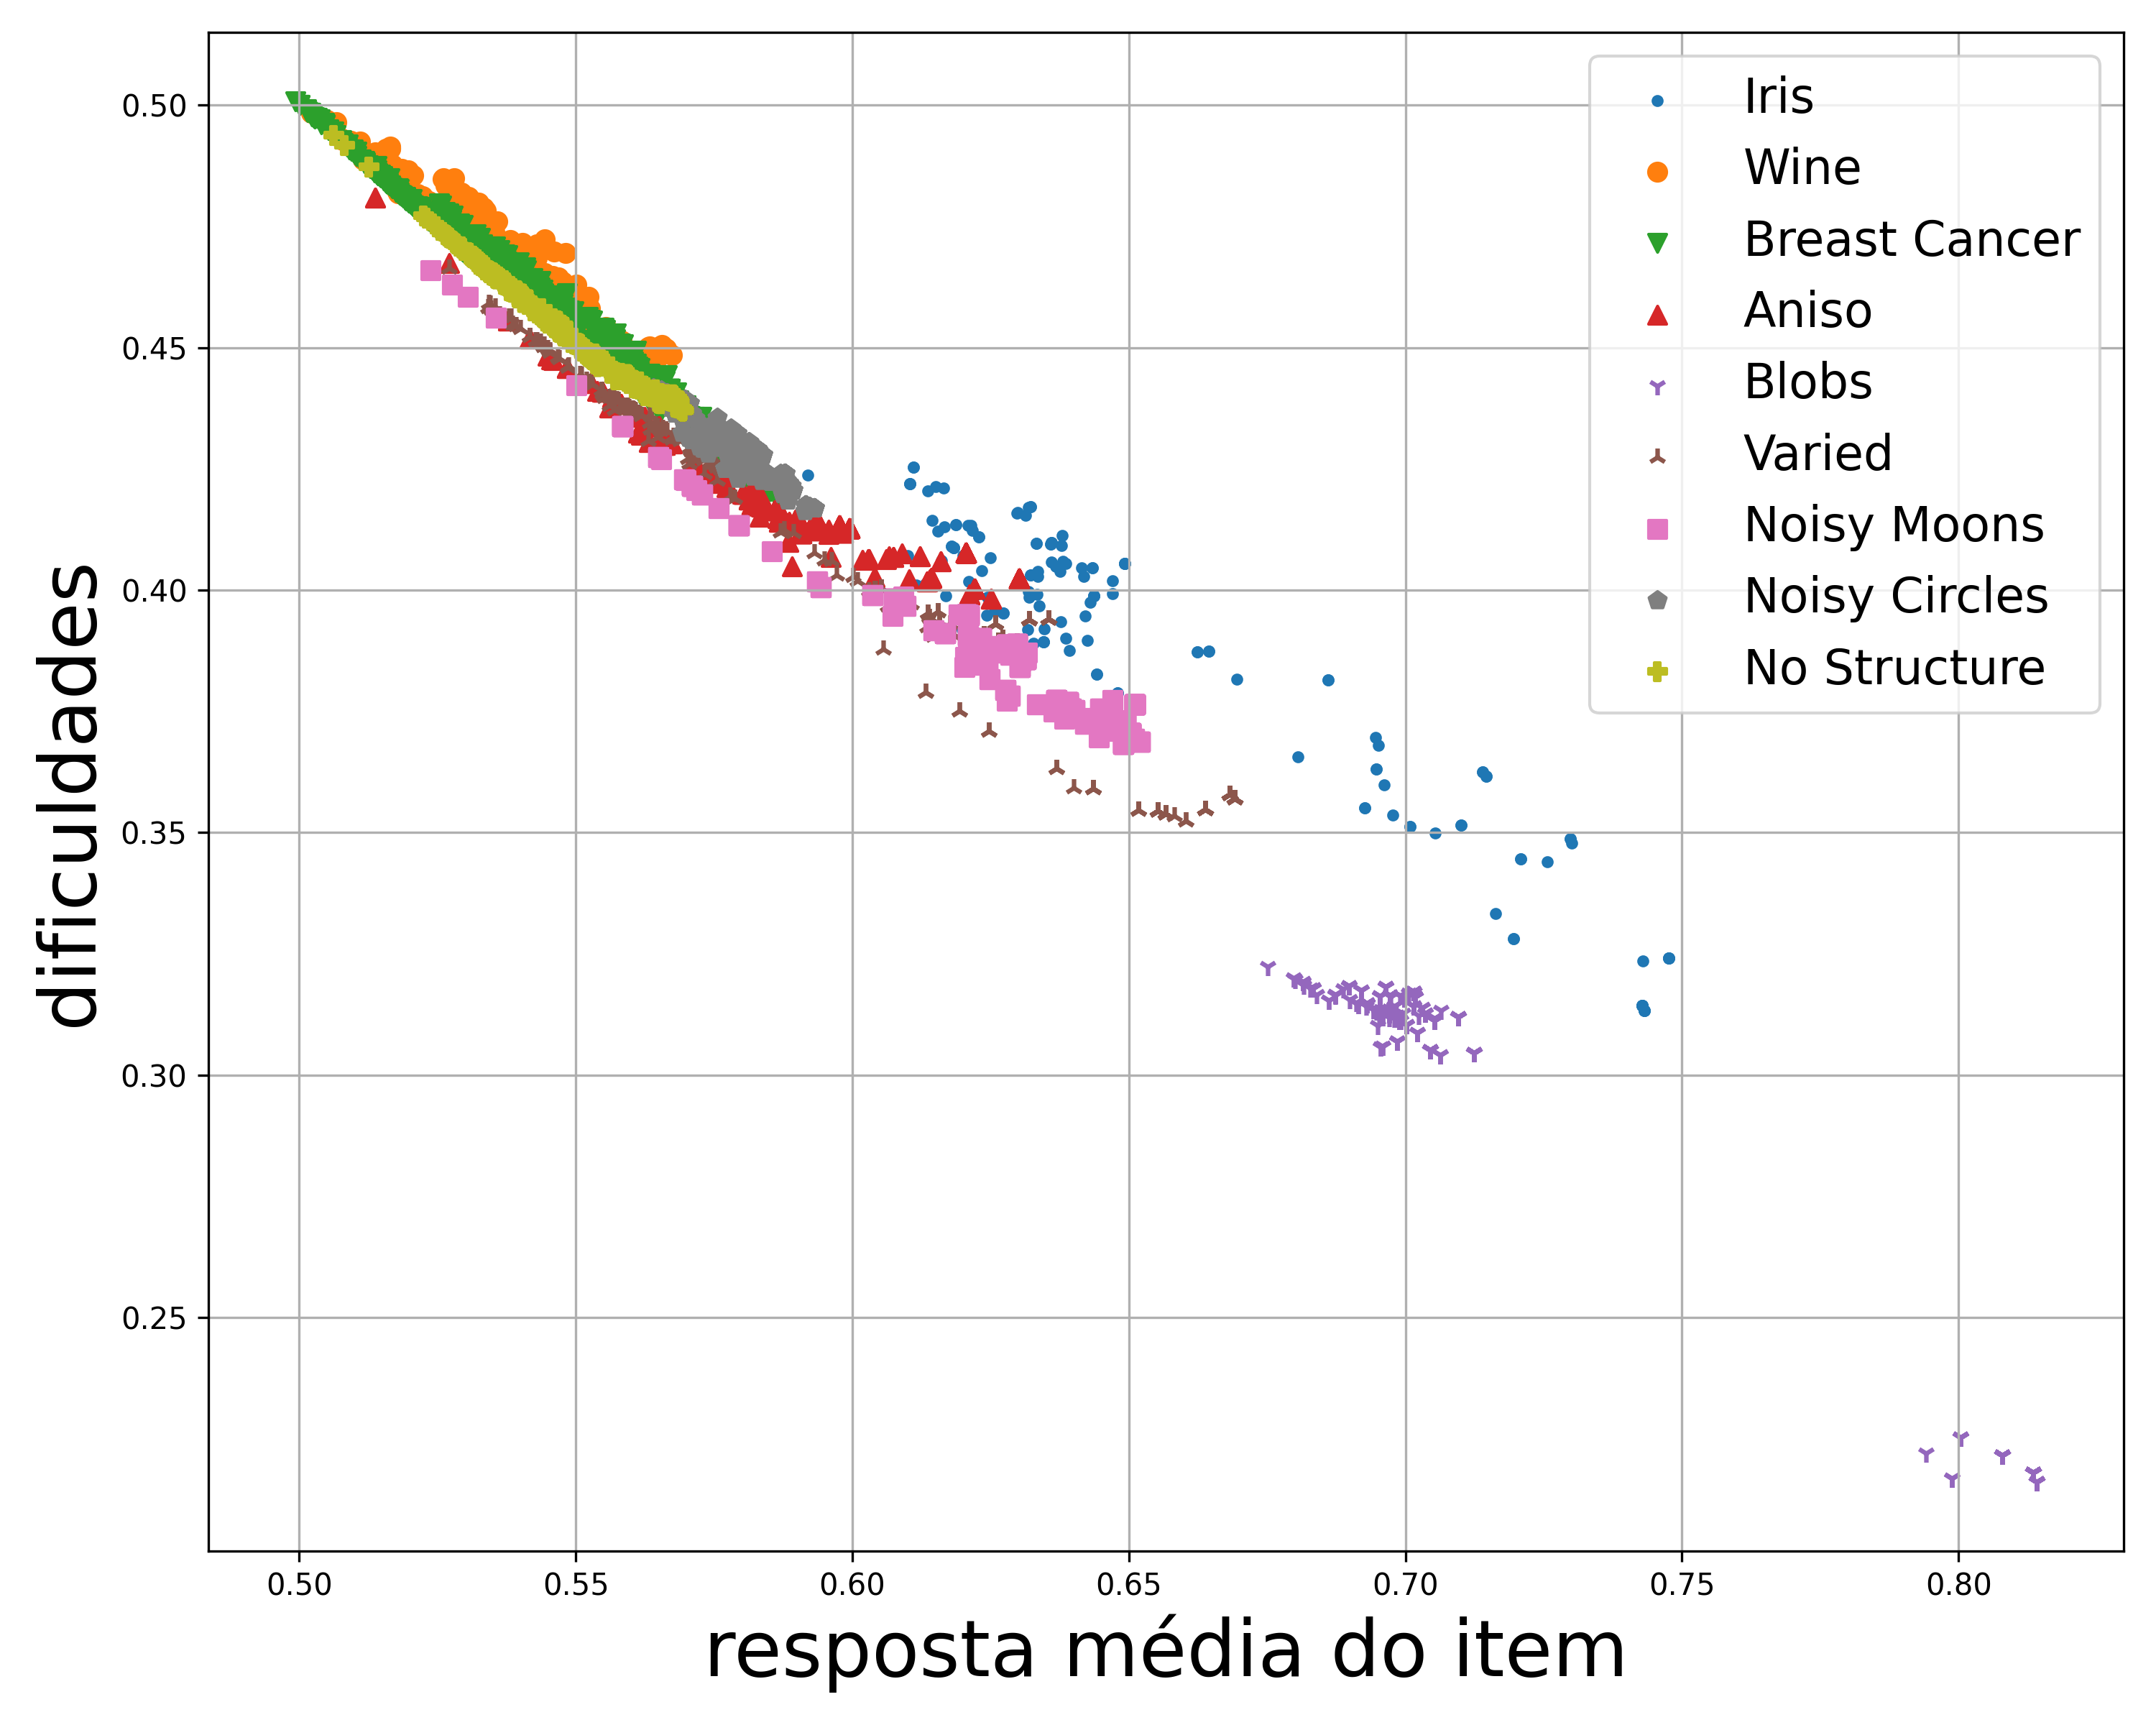
\includegraphics[width=\linewidth]{chapters/fundamentacao/imagens/random_n0_diff_versus_all.png}
    \end{minipage}
    \caption{Habilidades representadas em função das respostas médias dos modelos (esquerda) e dificuldades representadas graficamente em função das respostas médias dos itens (direita) para todos os conjuntos de dados.}   
    % \caption{Abilities versus average model response  (first row) and difficulties versus average item response (second row), and Pearson correlation coefficient ($\rho$), estimated for each model and each instance for Noisy Moons and Breast Cancer (without random partitions).}
    \label{fig:combined_figures}
\end{figure}

\begin{figure}[!htp]
    \centering
    \begin{subfigure}[t]{0.45\textwidth}
        \resizebox{0.9\textwidth}{!}{%
            % \begin{figure}
%     \centering
    \begin{tikzpicture}
        \begin{axis}[
            axis lines = left,
            xlabel = $\theta$,
            ylabel = {$E[p_{ij}]$},
            xmin = 0,
            xmax = 1,
            ymin = 0,
            ymax = 1
        ]
        \addplot [
            domain=1e-4:1-1e-4, 
            samples=100, 
            color=red,
        ]
        {1 / (1 + (0.352373 / (1 - 0.352373))^0.922765 * (x / (1 - x))^-0.922765)};
        
        \addplot[color=red]
        coordinates {
            (0.352373, 0) (0.352373, 0.5)
        };
        
        \addplot[color=black,mark=x,only marks]
        coordinates {
(0.3751986, 0.5160910055404927)
(0.48902684, 0.6939172462572203)
(0.51602244, 0.7539196039137098)
(0.514754, 0.7567487917010491)
(0.4988078, 0.7567487917010491)
(0.49516973, 0.7563362018153955)
(0.4917406, 0.7525050100200401)
(0.48559776, 0.751503006012024)
(0.48368728, 0.7371802428386184)
(0.5041737, 0.7453141577272191)
(0.38039544, 0.526111045620653)
(0.3775237, 0.5212189084050454)
(0.3764136, 0.5178592479075799)
(0.3764136, 0.5178592479075799)
(0.3751986, 0.5160910055404927)
(0.3751986, 0.5160910055404927)
(0.3751986, 0.5160910055404927)
(0.3751986, 0.5160910055404927)
(0.490017, 0.6904397029352823)
(0.5158445, 0.754214310974891)
(0.5153474, 0.7565130260521042)
(0.4983802, 0.7565130260521042)
(0.5097604, 0.7556289048685606)
(0.4906732, 0.7540964281504184)
(0.4976218, 0.7473771071554874)
(0.3751986, 0.5160910055404927)
(0.48614028, 0.7096546033242956)
(0.515595, 0.7516208888364965)
(0.49091965, 0.7516208888364965)
(0.4650427, 0.6278439231403985)
(0.46879038, 0.6258988565366026)
(0.4602671, 0.5107862784392314)
(0.44862637, 0.5107862784392314)
(0.51657873, 0.7536248968525285)
(0.45965382, 0.6768242367087115)
(0.4560667, 0.6576345969249423)
(0.51992995, 0.7567487917010491)
        };
        
        \end{axis}
    \end{tikzpicture}
%     \caption{Dataset \textit{volcanoes-b6}: minimum difficulty.}
%     \label{fig:easy_dataset}
% \end{figure}




        }
        \caption{Instância mais facil.}
        \label{fig:easy_dataset}
    \end{subfigure}
    \hfill
    \begin{subfigure}[t]{0.45\textwidth}
        \resizebox{0.9\textwidth}{!}{%
            % \begin{figure}
%     \centering
    \begin{tikzpicture}
        \begin{axis}[
            axis lines = left,
            xlabel = $\theta$,
            ylabel = {$E[p_{ij}]$},
            xmin = 0,
            xmax = 1,
            ymin = 0,
            ymax = 1
        ]
        \addplot [
            domain=1e-4:1-1e-4, 
            samples=100, 
            color=red,
        ]
        {1 / (1 + (0.466350 / (1 - 0.466350))^0.830393 * (x / (1 - x))^-0.830393)};
        
        \addplot[color=red]
        coordinates {
            (0.466350, 0) (0.466350, 0.5)
        };
        
        \addplot[color=black,mark=x,only marks]
        coordinates {
           (0.3751986, 0.4163621360367794)
(0.48902684, 0.4945773900742661)
(0.51602244, 0.4829069904514912)
(0.514754, 0.6128728044323942)
(0.4988078, 0.6112224448897795)
(0.49516973, 0.5901214193092067)
(0.4917406, 0.5736767652952964)
(0.48559776, 0.5964281504184841)
(0.48368728, 0.5559354002121891)
(0.5041737, 0.5594718849463634)
(0.38039544, 0.4223741600848756)
(0.3775237, 0.4181893198161028)
(0.3764136, 0.4178946127549216)
(0.3764136, 0.4178946127549216)
(0.3751986, 0.4163621360367794)
(0.3751986, 0.4163621360367794)
(0.3751986, 0.4163621360367794)
(0.3751986, 0.4163621360367794)
(0.490017, 0.4961688082046446)
(0.5158445, 0.5854650477425439)
(0.5153474, 0.6129317458446304)
(0.4983802, 0.6024991158788164)
(0.5097604, 0.5777437227395968)
(0.4906732, 0.577507957090652)
(0.4976218, 0.5942473181657433)
(0.3751986, 0.4163621360367794)
(0.48614028, 0.5058351998113875)
(0.515595, 0.4725333018979135)
(0.49091965, 0.5636567252151361)
(0.4650427, 0.5793940822822115)
(0.46879038, 0.6144052811505364)
(0.4602671, 0.6144052811505364)
(0.44862637, 0.6141105740893552)
(0.51657873, 0.5870564658729223)
(0.45965382, 0.5134975834020983)
(0.4560667, 0.5246627709199914)
(0.51992995, 0.6144052811505364)
        };
        
        \end{axis}
    \end{tikzpicture}
        }
        \caption{Instância mais dificil.}
        \label{fig:hard_class_dataset}
    \end{subfigure}
    \caption{\gls{CCI}s das instâncias mais faceis e mais dificeis para o conjunto de dados Varied.}\label{fig:easy:hard:clas}
\end{figure}

Por fim, a Figura \ref{fig:combined_figures} apresenta os gráficos das habilidades e dificuldades estimadas em função das respostas médias dos modelos e das instâncias, respectivamente. No caso das habilidades, observa-se que cada conjunto de dados forma uma espécie de "faixa" aproximadamente linear, sugerindo forte correlação entre a média de concordância e a habilidade latente estimada. Ainda assim, em conjuntos mais complexos, como Noisy Moons e Breast Cancer, valores semelhantes de habilidade podem estar associados a médias de resposta distintas, evidenciando que a relação não é perfeitamente uniforme.

Esse efeito torna ainda mais evidente quando se analisam as dificuldades em comparação com as respostas médias das instâncias, tanto em conjuntos simples quanto complexos. De modo geral, as médias funcionam como uma boa aproximação do comportamento das variáveis latentes estimadas pelo $\beta^{4}$-\gls{IRT}, mas não capturam integralmente a estrutura modelada, indicando que a abordagem baseada em \gls{TRI} fornece uma aproximação mais rica do desempenho de modelos e da complexidade das instâncias.


\section{Correlação entre o \gls{CLAIRE} e métricas de validação}

Os resultados apresentaram uma forte correlação entre a  habilidade estimada pelo método do \gls{CLAIRE} e as métricas de validação externa \gls{ARI} para todos conjuntos de dados, o qual é esperado, uma vez que o \gls{ARI} é também calculado baseado se pares de instâncias são agrupadas juntas ou não. De maneira similar, a habilidade e a métrica \gls{v} estavam fortemente correlacionadas postivamente para todos os conjuntos, excepto para o Aniso. Por outro lado, para a maioria dos conjuntos, a habilidade não era fortemente correlacionada com a \gls{MI}. Isso provavelmente se deu devido ao \gls{MI} tender a favorecer modelos com alto número de clusters, independentemente de outros caracteristicas de agrupamento \cite{gates2017impact}. Esses resultados são fundamentais para a validação do método proposto, uma vez que o \gls{CLAIRE} baseia-se exclusivamente na concordância entre os modelos do conjunto e, ainda assim, consegue gerar ranqueamentos próximos aos obtidos por índices de validação externa, os quais utilizam a verdade de referência para avaliar o desempenho dos algoritmos de agrupamento.

\begin{figure}[!htb]
    \centering
    \includegraphics[width=0.9\textwidth]{chapters/fundamentacao/imagens/random_n0_abilities_corr_spearman.png}
    \caption{Correlação entre habilidade e outros índices.}
    \label{fig:abilities_corr_spearman}
\end{figure}

Considerando os índices internos de validação, as habilidades estimadas pelo \gls{CLAIRE} também apresentam correlação positiva a moderada, e forte nos conjuntos Iris, Wine, Breast Cancer, Blobs e Varied, com os escores de CH e Silhouette, além de correlação negativa com o índice \gls{DB}. Um comportamento inverso é observado no conjunto Noisy Moons. Esse padrão é compatível com o fato de que cada índice interno costuma apresentar algum viés em relação a determinadas estruturas de clusters (como número de grupos, tamanhos relativos, separabilidade, compacidade ou presença de ruído). Assim, características específicas do conjunto de dados podem favorecer índices cujo viés esteja alinhado a tais propriedades.

De modo geral, a maior variabilidade verificada entre os índices internos indica que alguns deles podem não ser adequados para avaliar modelos sob determinadas estruturas de dados. Por essa razão, o \gls{CLAIRE} tende a produzir ranqueamentos mais próximos daqueles obtidos por índices externos do que pelos próprios índices internos.


\section{Efeito da partição aleatoria no grupo de modelos}\label{sec:part_random}

Nesta seção, analisamos o efeito da inclusão de modelos aleatórios no conjunto sobre os ranqueamentos produzidos pelo \gls{CLAIRE}. Para isso, foram geradas partições aleatórias para cada dataset, atribuindo cada instância, de forma randômica, a um dos $K$ clusters, sendo $K$ igual ao número de grupos da verdade de referência. Essas partições foram então adicionadas progressivamente ao conjunto de modelos, e novos ranqueamentos foram obtidos por meio do \gls{CLAIRE}. A Figura \ref{fig:simulation} apresenta os resultados para os conjuntos Noisy Moons e Breast Cancer, à medida que o número de partições aleatórias varia de $0$ a $35$ (Essas  artições não contribuem para as métricas de Average e Best Responses).


\begin{figure}[htbp]
\centering
\begin{minipage}{.83\textwidth}
  \centering
  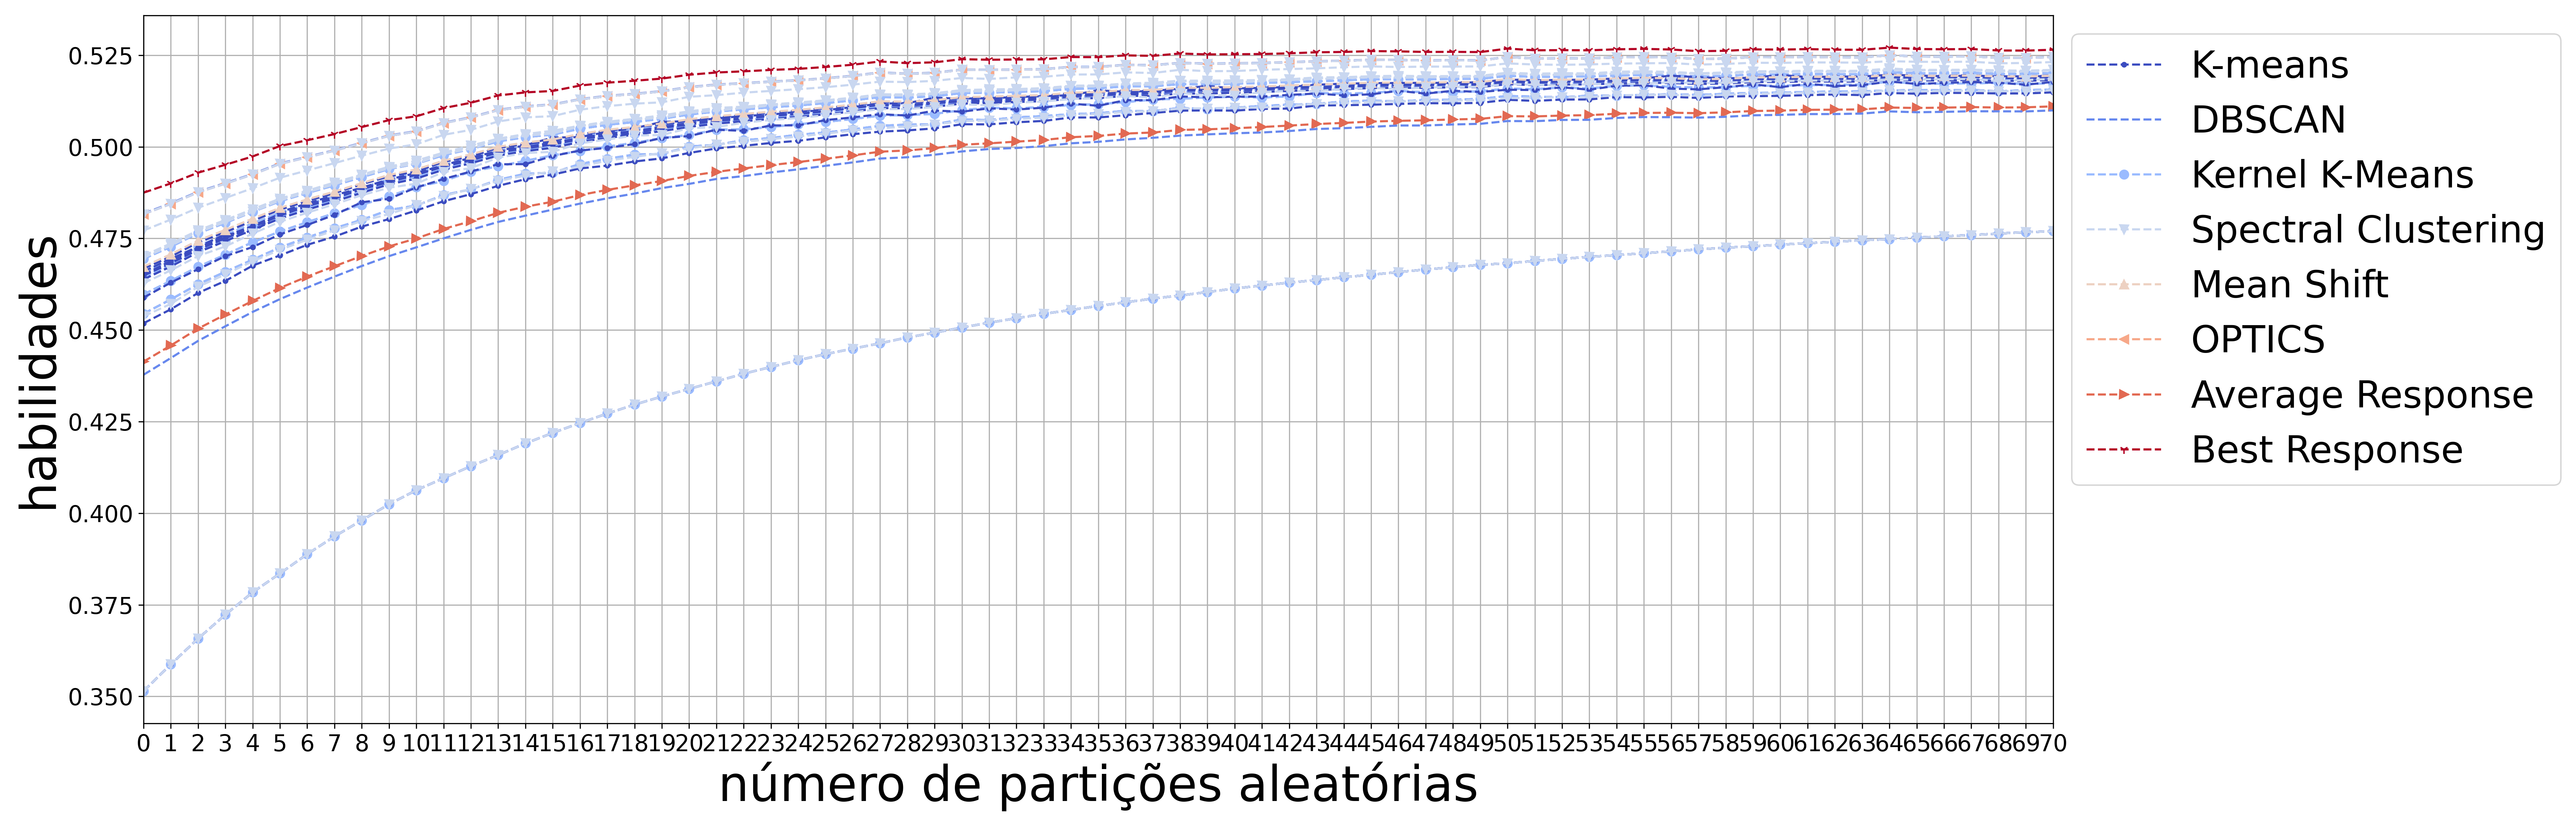
\includegraphics[width=\linewidth]{chapters/fundamentacao/imagens/noisy_moons.png}
  % \caption{Simulation involving the noisy moons dataset (estimated abilities for each increment of a random partition)}
  %\label{fig:simu_noisy_moons}
\end{minipage}%
\hspace{.05\textwidth}%
\begin{minipage}{.83\textwidth}
  \centering
  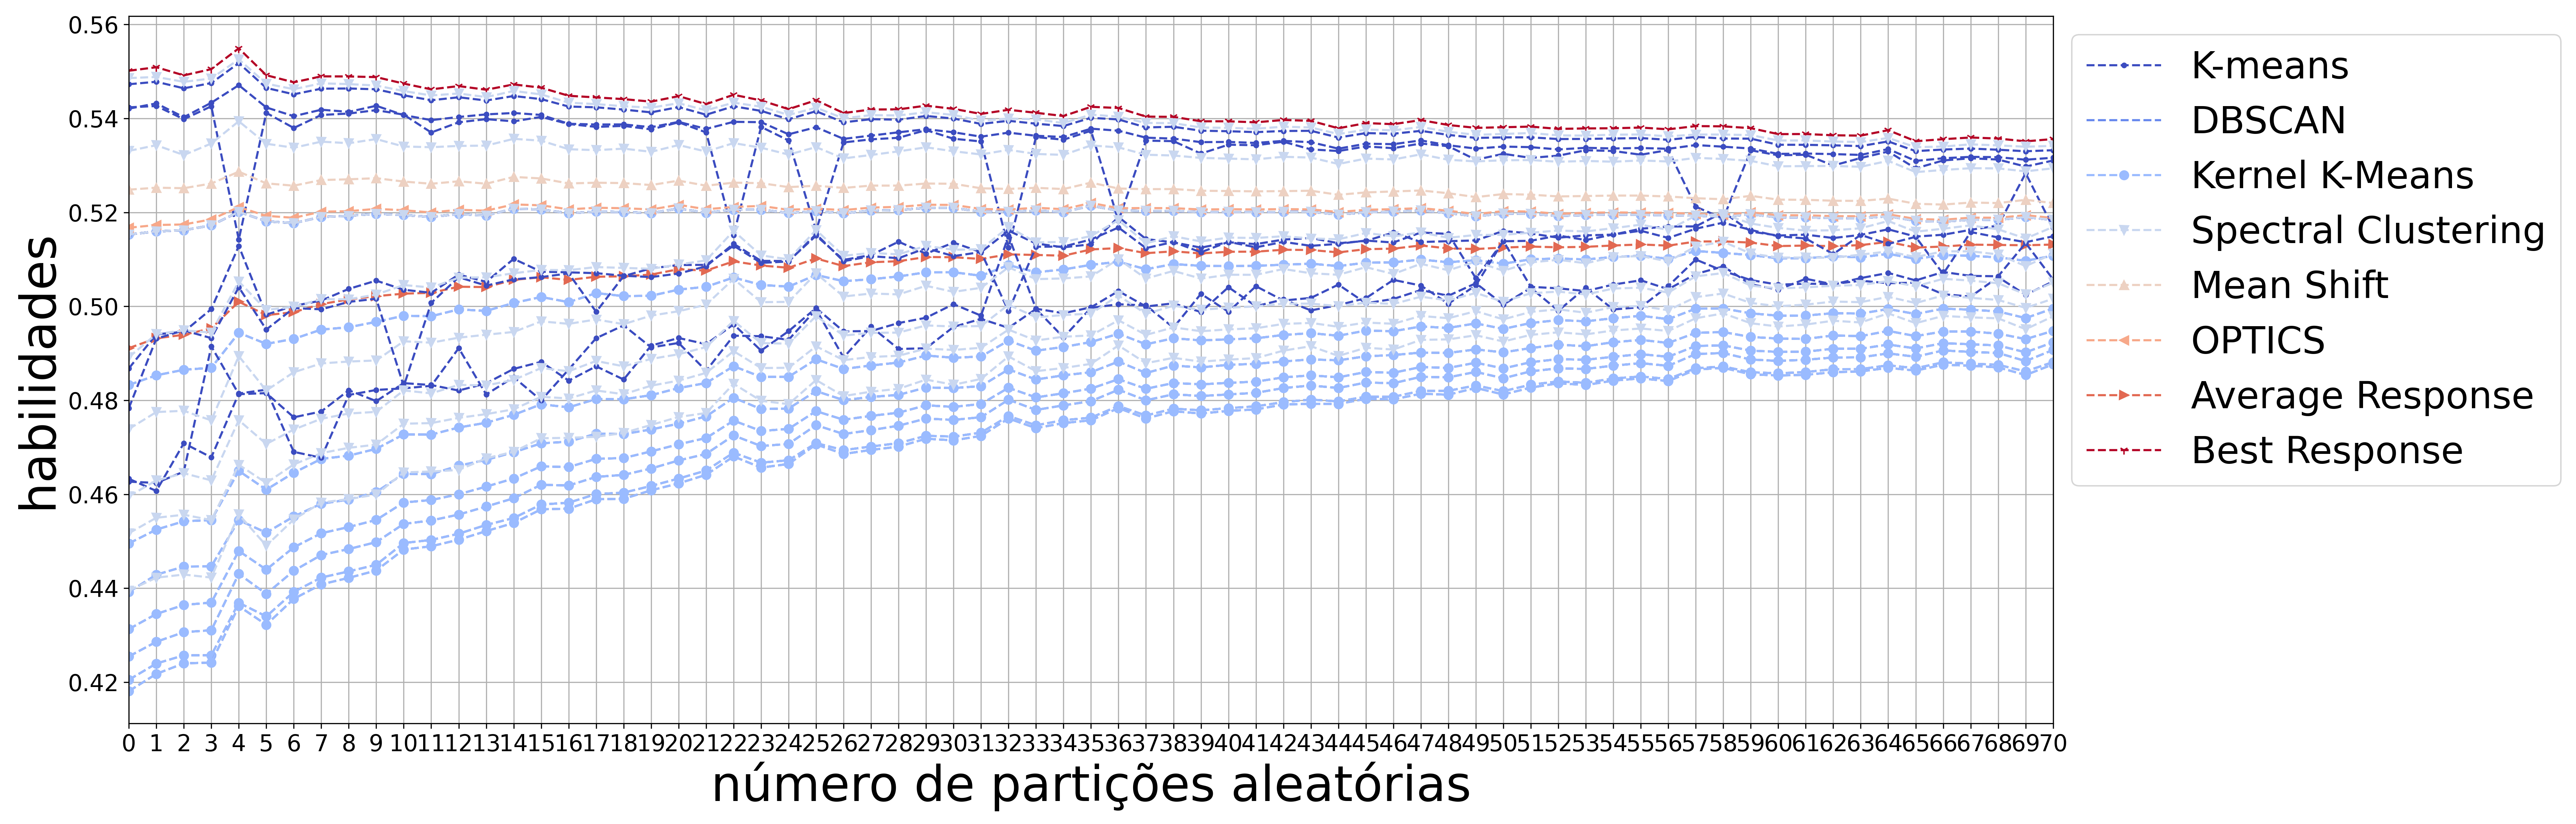
\includegraphics[width=\linewidth]{chapters/fundamentacao/imagens/breast_cancer.png}
  % \caption{Simulation involving the breast cancer dataset (estimated abilities for each increment of a random partition)}
  %\label{fig:simu_breast}
\end{minipage}
\caption{Classificações geradas pelo \gls{CLAIRE} para Noisy Moons (acima) e Câncer de Mama (abaixo) conforme o número de partições aleatórias no conjunto de modelos aumenta de $0$ para $35$.}
\label{fig:simulation}
\end{figure}


Embora se observe aumento nos valores de algumas habilidades (ou mesmo em todas elas), no caso do Noisy Moons a ordenação relativa dos modelos tende a permanecer estável conforme cresce o número de partições aleatórias, em ambos os conjuntos analisados. No Breast Cancer, apenas algumas versões do K-Means apresentam pequenas oscilações, possivelmente atribuídas à variabilidade inerente ao processo de estimação das variáveis latentes. Esse comportamento robusto, com ranqueamentos essencialmente preservados ou sofrendo alterações pontuais, também foi verificado nos demais conjuntos (ver Apêndice \ref{chp:appendice_b}). Assim, os resultados indicam que o \gls{CLAIRE} mantém sua capacidade de produzir ranqueamentos informativos mesmo diante da presença de múltiplos modelos aleatórios no conjunto.

\section{Ánalise da estabilidade da habilidade}

Conforme discutido na Seção \ref{sec:agree_correctness}, o \gls{CLAIRE} parte do pressuposto de que a habilidade de concordância constitui uma estratégia adequada para avaliar agrupamentos, assumindo que a maioria dos modelos considerados é capaz de produzir partições significativas para o conjunto de dados. Uma forma de examinar essa hipótese consiste em analisar a estabilidade das habilidades estimadas. Para isso, adotou-se um procedimento \gls{LOO}, no qual, a cada etapa, um respondente (ou seja, um modelo) é removido do conjunto e o \gls{CLAIRE} é novamente executado para reestimar as habilidades. Caso o método seja robusto em relação ao conjunto de modelos, espera-se que as habilidades permaneçam praticamente inalteradas. O procedimento pode ser descrito da seguinte forma:

\begin{itemize}
    \item[1] remover o modelo de agrupamento $A$ do conjunto de respondentes;
    
    \item[2] executar novamente o \gls{CLAIRE} com os modelos restantes e estimar suas habilidades;
    
    \item[3] avaliar a estabilidade da habilidade de cada modelo remanescente $B$, calculando a diferença entre sua habilidade antes e depois da remoção de $A$;
    
    \item[4] repetir esse processo para todos os modelos.
\end{itemize}

As Tabelas \ref{tab:metrics_iris_wine_breastcancer} a \ref{tab:metrics_noisy_circles_no_structure} apresentam os resultados dessa análise. Para cada modelo, são reportadas a média e a amplitude (valor máximo menos valor mínimo) da variação na habilidade dos demais modelos quando ele é retirado do conjunto.

De modo geral, as diferenças observadas são muito pequenas e, em média, próximas de $0$, evidenciando a robustez da abordagem. Amplitudes ligeiramente maiores aparecem quando o modelo com maior concordância em determinado conjunto é removido  (como K-means e Kernel K-means com $K=3$ no caso do Blobs) pois sua exclusão reduz o nível global de concordância no conjunto. As menores amplitudes são verificadas no dataset No Structure, cuja ausência de estrutura de clusters implica que nenhum dos modelos se ajusta adequadamente aos dados.

\begin{table*}[!t]
    \centering
    \tiny
    \caption{Média e intervalo da diferença de habilidades depois de remover cada modelo do grupo de modelos para os conjuntos Iris, Wine e Breast Cancer.}
    \label{tab:metrics_iris_wine_breastcancer}
    \begin{tabular}{l|c|ll|ll|ll}
    \midrule
     &  & \multicolumn{2}{c|}{Iris} & \multicolumn{2}{c|}{Wine} & \multicolumn{2}{c}{Breast Cancer} \\
      Modelo   & Versão & Média & $\Delta_{\max-\min}$ & Média & $\Delta_{\max-\min}$ & Média & $\Delta_{\max-\min}$ \\
    \midrule
    Mean Shift & -- & -0.001 & 0.009 & -0.000 & 0.004 & -0.001 & 0.007 \\
    \midrule
    \multirow[t]{6}{*}{OPTICS} & -- & -0.001 & 0.009 & -0.000 & 0.004 & -0.001 & 0.007 \\
    \midrule
    \multirow[t]{9}{*}{DBSCAN} & $\epsilon=0.1$ & -0.001 & 0.012 & -0.000 & 0.004 & -0.001 & 0.007 \\
     & $\epsilon=0.2$ & -0.001 & 0.009 & -0.000 & 0.004 & -0.001 & 0.007 \\
     & $\epsilon=0.3$ & -0.001 & 0.007 & -0.000 & 0.004 & -0.001 & 0.007 \\
     & $\epsilon=0.4$ & -0.001 & 0.007 & -0.000 & 0.004 & -0.001 & 0.007 \\
     & $\epsilon=0.5$ & -0.001 & 0.008 & -0.000 & 0.004 & -0.001 & 0.007 \\
     & $\epsilon=0.6$ & -0.001 & 0.009 & -0.000 & 0.004 & -0.001 & 0.007 \\
     & $\epsilon=0.7$ & -0.001 & 0.009 & -0.000 & 0.004 & -0.001 & 0.007 \\
     & $\epsilon=0.8$ & -0.001 & 0.009 & -0.000 & 0.004 & -0.001 & 0.007 \\
     & $\epsilon=0.9$ & -0.001 & 0.009 & -0.000 & 0.004 & -0.001 & 0.007 \\
    \midrule
    \multirow[t]{8}{*}{K-means} & $K=1$ & -0.001 & 0.012 & -0.000 & 0.004 & -0.001 & 0.007 \\
     & $K=2$ & -0.001 & 0.009 & -0.000 & 0.005 & -0.001 & 0.007 \\
     & $K=3$ & -0.001 & 0.009 & -0.000 & 0.005 & -0.001 & 0.007 \\
     & $K=4$ & -0.001 & 0.009 & -0.000 & 0.004 & -0.001 & 0.006 \\
     & $K=5$ & -0.001 & 0.009 & -0.000 & 0.005 & -0.001 & 0.007 \\
     & $K=6$ & -0.001 & 0.009 & -0.000 & 0.004 & -0.000 & 0.006 \\
     & $K=7$ & -0.001 & 0.009 & -0.000 & 0.003 & -0.000 & 0.006 \\
     & $K=8$ & -0.001 & 0.008 & -0.000 & 0.003 & -0.000 & 0.006 \\
    \midrule
    \multirow[t]{8}{*}{Kernel K-means} & $K=1$ & -0.001 & 0.012 & -0.000 & 0.004 & -0.001 & 0.007 \\
     & $K=2$ & -0.001 & 0.009 & -0.000 & 0.003 & -0.000 & 0.005 \\
     & $K=3$ & -0.001 & 0.009 & -0.000 & 0.003 & -0.000 & 0.006 \\
     & $K=4$ & -0.001 & 0.009 & -0.000 & 0.003 & -0.000 & 0.006 \\
     & $K=5$ & -0.001 & 0.009 & -0.000 & 0.003 & -0.000 & 0.006 \\
     & $K=6$ & -0.001 & 0.008 & -0.000 & 0.004 & -0.000 & 0.006 \\
     & $K=7$ & -0.001 & 0.009 &  0.000 & 0.004 & -0.000 & 0.006 \\
     & $K=8$ & -0.001 & 0.008 &  0.000 & 0.004 & -0.000 & 0.006 \\
    \midrule
    \multirow[t]{8}{*}{Spectral Clustering} & $K=1$ & -0.001 & 0.012 & -0.000 & 0.004 & -0.001 & 0.007 \\
     & $K=2$ & -0.001 & 0.009 & -0.000 & 0.005 & -0.001 & 0.006 \\
     & $K=3$ & -0.001 & 0.009 & -0.000 & 0.005 & -0.001 & 0.006 \\
     & $K=4$ & -0.001 & 0.009 & -0.000 & 0.005 & -0.001 & 0.006 \\
     & $K=5$ & -0.001 & 0.009 & -0.000 & 0.005 & -0.001 & 0.006 \\
     & $K=6$ & -0.001 & 0.009 & -0.000 & 0.004 & -0.000 & 0.006 \\
     & $K=7$ & -0.001 & 0.009 & -0.000 & 0.004 & -0.000 & 0.006 \\
     & $K=8$ & -0.001 & 0.008 & -0.000 & 0.004 & -0.000 & 0.006 \\
    \midrule
    \end{tabular}
\end{table*}

\begin{table*}[!t]
    \centering
    \tiny
    \caption{Média e intervalo da diferença de habilidades depois de remover cada modelo do grupo de modelos para os conjuntos Aniso e Blobs.}
    \label{tab:metrics_aniso_blobs}
    \begin{tabular}{l|c|ll|ll}
    \midrule
     & & \multicolumn{2}{c|}{Aniso} & \multicolumn{2}{c}{Blobs} \\
          Modelo & Versão & Média & $\Delta_{\max-\min}$ & Média & $\Delta_{\max-\min}$ \\
    \midrule
    Mean Shift      & -- & -0.000 & 0.005 & -0.001 & 0.030 \\
    \midrule
    \multirow[t]{6}{*}{OPTICS}
      & - & -0.000 & 0.005 & -0.001 & 0.030 \\
    \midrule
    \multirow[t]{9}{*}{DBSCAN} 
      & $\epsilon=0.1$ & -0.000 & 0.005 & -0.001 & 0.028 \\
      & $\epsilon=0.2$ & -0.000 & 0.005 & -0.001 & 0.030 \\
      & $\epsilon=0.3$ & -0.000 & 0.006 & -0.001 & 0.030 \\
      & $\epsilon=0.4$ & -0.000 & 0.006 & -0.001 & 0.030 \\
      & $\epsilon=0.5$ & -0.000 & 0.006 & -0.001 & 0.018 \\
      & $\epsilon=0.6$ & -0.000 & 0.006 & -0.001 & 0.018 \\
      & $\epsilon=0.7$ & -0.000 & 0.006 & -0.001 & 0.018 \\
      & $\epsilon=0.8$ & -0.000 & 0.006 & -0.001 & 0.018 \\
      & $\epsilon=0.9$ & -0.000 & 0.006 & -0.001 & 0.018 \\
    \midrule
    \multirow[t]{8}{*}{K-means} 
      & $K=1$ & -0.000 & 0.006 &  0.000 & 0.023 \\
      & $K=2$ & -0.000 & 0.005 & -0.001 & 0.018 \\
      & $K=3$ & -0.000 & 0.005 & -0.001 & 0.030 \\
      & $K=4$ & -0.000 & 0.005 & -0.001 & 0.023 \\
      & $K=5$ & -0.000 & 0.005 & -0.001 & 0.017 \\
      & $K=6$ & -0.000 & 0.005 & -0.001 & 0.017 \\
      & $K=7$ & -0.000 & 0.005 & -0.001 & 0.012 \\
      & $K=8$ & -0.000 & 0.005 & -0.001 & 0.016 \\
    \midrule
    \multirow[t]{8}{*}{Kernel K-means} 
      & $K=1$ & -0.000 & 0.006 &  0.000 & 0.023 \\
      & $K=2$ & -0.000 & 0.005 & -0.001 & 0.018 \\
      & $K=3$ & -0.000 & 0.005 & -0.001 & 0.030 \\
      & $K=4$ & -0.000 & 0.005 & -0.001 & 0.028 \\
      & $K=5$ & -0.000 & 0.005 & -0.001 & 0.021 \\
      & $K=6$ & -0.000 & 0.005 & -0.001 & 0.017 \\
      & $K=7$ & -0.000 & 0.005 & -0.001 & 0.019 \\
      & $K=8$ & -0.000 & 0.005 & -0.001 & 0.026 \\
    \midrule
    \multirow[t]{8}{*}{Spectral Clustering} 
      & $K=1$ & -0.000 & 0.006 &  0.000 & 0.023 \\
      & $K=2$ & -0.000 & 0.005 & -0.001 & 0.011 \\
      & $K=3$ & -0.000 & 0.005 & -0.000 & 0.008 \\
      & $K=4$ & -0.000 & 0.005 & -0.001 & 0.014 \\
      & $K=5$ & -0.000 & 0.005 & -0.001 & 0.012 \\
      & $K=6$ & -0.000 & 0.005 & -0.001 & 0.014 \\
      & $K=7$ & -0.000 & 0.005 & -0.001 & 0.014 \\
      & $K=8$ & -0.000 & 0.005 & -0.001 & 0.012 \\
    \midrule
    \end{tabular}
\end{table*}

\begin{table*}[!t]
    \centering
    \tiny
    \caption{Média e intervalo da diferença de habilidades depois de remover cada modelo do grupo de modelos para os conjuntos  Varied e Noisy Moons.}
    \label{tab:metrics_varied_noisy_moons}
    \begin{tabular}{l|c|ll|ll}
    \midrule
    Modelo & Versão 
      & \multicolumn{2}{c|}{Varied} 
      & \multicolumn{2}{c}{Noisy Moons} \\
          &        
      & Média & $\Delta_{\max-\min}$ 
      & Média & $\Delta_{\max-\min}$ \\
    \midrule
    Mean Shift      & -- & -0.001 & 0.008 & -0.000 & 0.006 \\
    \midrule
    \multirow[t]{6}{*}{OPTICS} 
      & -- & -0.000 & 0.006 & -0.000 & 0.006    \\
    \midrule
    \multirow[t]{9}{*}{DBSCAN} 
      & $\epsilon=0.1$ & -0.000 & 0.007 & -0.000 & 0.007 \\
      & $\epsilon=0.2$ & -0.001 & 0.007 & -0.000 & 0.006 \\
      & $\epsilon=0.3$ & -0.000 & 0.007 & -0.000 & 0.006 \\
      & $\epsilon=0.4$ & -0.000 & 0.007 & -0.000 & 0.006 \\
      & $\epsilon=0.5$ & -0.000 & 0.007 & -0.000 & 0.006 \\
      & $\epsilon=0.6$ & -0.000 & 0.007 &  0.000 & 0.010 \\
      & $\epsilon=0.7$ & -0.000 & 0.007 &  0.000 & 0.010 \\
      & $\epsilon=0.8$ & -0.000 & 0.007 &  0.000 & 0.010 \\
      & $\epsilon=0.9$ & -0.000 & 0.007 &  0.000 & 0.010 \\
    \midrule
    \multirow[t]{8}{*}{K-means} 
      & $K=1$ & -0.000 & 0.007 & -0.000 & 0.010 \\
      & $K=2$ & -0.000 & 0.007 & -0.000 & 0.006 \\
      & $K=3$ & -0.001 & 0.008 & -0.000 & 0.006 \\
      & $K=4$ & -0.001 & 0.008 & -0.000 & 0.006 \\
      & $K=5$ & -0.001 & 0.008 & -0.000 & 0.006 \\
      & $K=6$ & -0.000 & 0.007 & -0.000 & 0.006 \\
      & $K=7$ & -0.000 & 0.006 & -0.000 & 0.006 \\
      & $K=8$ & -0.000 & 0.006 & -0.000 & 0.007 \\
    \midrule
    \multirow[t]{8}{*}{Kernel K-means} 
      & $K=1$ & -0.000 & 0.007 &  0.000 & 0.010 \\
      & $K=2$ & -0.000 & 0.007 & -0.000 & 0.006 \\
      & $K=3$ & -0.001 & 0.008 & -0.000 & 0.006 \\
      & $K=4$ & -0.001 & 0.008 & -0.000 & 0.006 \\
      & $K=5$ & -0.000 & 0.007 & -0.000 & 0.006 \\
      & $K=6$ & -0.001 & 0.008 & -0.000 & 0.006 \\
      & $K=7$ & -0.000 & 0.007 & -0.000 & 0.006 \\
      & $K=8$ & -0.001 & 0.007 & -0.000 & 0.007 \\
    \midrule
    \multirow[t]{8}{*}{Spectral Clustering} 
      & $K=1$ & -0.000 & 0.007 & -0.000 & 0.010 \\
      & $K=2$ & -0.000 & 0.007 & -0.000 & 0.006 \\
      & $K=3$ & -0.001 & 0.008 & -0.000 & 0.006 \\
      & $K=4$ & -0.000 & 0.007 & -0.000 & 0.006 \\
      & $K=5$ & -0.000 & 0.006 & -0.000 & 0.006 \\
      & $K=6$ & -0.000 & 0.006 & -0.000 & 0.006 \\
      & $K=7$ & -0.000 & 0.006 & -0.000 & 0.006 \\
      & $K=8$ & -0.000 & 0.007 & -0.000 & 0.007 \\
    \midrule
    \end{tabular}
\end{table*}

\begin{table*}[!t]
    \centering
    \tiny
    \caption{Média e intervalo da diferença de habilidades depois de remover cada modelo do grupo de modelos para os conjuntos Noisy Circles e No Structure.}
    \label{tab:metrics_noisy_circles_no_structure}
    \begin{tabular}{l|c|ll|ll}
    \midrule
    Modelo & Versão 
      & \multicolumn{2}{c|}{Noisy Circles} 
      & \multicolumn{2}{c}{No Structure} \\
          &        
      & Média & $\Delta_{\max-\min}$ 
      & Média & $\Delta_{\max-\min}$ \\
    \midrule
    Mean Shift      & -- & -0.000 & 0.005 & -0.000 & 0.004 \\
    \midrule
    \multirow[t]{6}{*}{OPTICS}
      & -- & -0.000 & 0.004 & -0.000 & 0.004     \\
    \midrule
    \multirow[t]{9}{*}{DBSCAN} 
      & $\epsilon=0.1$ & -0.000 & 0.005 &  0.000 & 0.003 \\
      & $\epsilon=0.2$ & -0.000 & 0.004 & -0.000 & 0.004 \\
      & $\epsilon=0.3$ & -0.000 & 0.004 & -0.000 & 0.004 \\
      & $\epsilon=0.4$ & -0.000 & 0.004 & -0.000 & 0.004 \\
      & $\epsilon=0.5$ & -0.000 & 0.004 & -0.000 & 0.004 \\
      & $\epsilon=0.6$ & -0.000 & 0.007 & -0.000 & 0.004 \\
      & $\epsilon=0.7$ & -0.000 & 0.007 & -0.000 & 0.004 \\
      & $\epsilon=0.8$ & -0.000 & 0.007 & -0.000 & 0.004 \\
      & $\epsilon=0.9$ & -0.000 & 0.007 & -0.000 & 0.004 \\
    \midrule
    \multirow[t]{8}{*}{K-means} 
      & $K=1$ & -0.000 & 0.007 & -0.000 & 0.004 \\
      & $K=2$ & -0.000 & 0.005 & -0.000 & 0.005 \\
      & $K=3$ & -0.000 & 0.005 &  0.000 & 0.005 \\
      & $K=4$ & -0.000 & 0.004 & -0.000 & 0.005 \\
      & $K=5$ & -0.000 & 0.005 & -0.000 & 0.005 \\
      & $K=6$ & -0.000 & 0.005 & -0.000 & 0.004 \\
      & $K=7$ & -0.000 & 0.005 & -0.000 & 0.004 \\
      & $K=8$ & -0.000 & 0.005 & -0.000 & 0.004 \\
    \midrule
    \multirow[t]{8}{*}{Kernel K-means} 
      & $K=1$ & -0.000 & 0.007 & -0.000 & 0.004 \\
      & $K=2$ & -0.000 & 0.005 & -0.000 & 0.004 \\
      & $K=3$ & -0.000 & 0.005 & -0.000 & 0.005 \\
      & $K=4$ & -0.000 & 0.004 & -0.000 & 0.005 \\
      & $K=5$ & -0.000 & 0.004 & -0.000 & 0.005 \\
      & $K=6$ & -0.000 & 0.004 & -0.000 & 0.004 \\
      & $K=7$ & -0.000 & 0.004 & -0.000 & 0.004 \\
      & $K=8$ & -0.000 & 0.004 & -0.000 & 0.004 \\
    \midrule
    \multirow[t]{8}{*}{Spectral Clustering} 
      & $K=1$ & -0.000 & 0.007 & -0.000 & 0.004 \\
      & $K=2$ & -0.000 & 0.004 & -0.000 & 0.005 \\
      & $K=3$ & -0.000 & 0.004 & -0.000 & 0.005 \\
      & $K=4$ & -0.000 & 0.004 & -0.000 & 0.006 \\
      & $K=5$ & -0.000 & 0.004 & -0.000 & 0.005 \\
      & $K=6$ & -0.000 & 0.004 & -0.000 & 0.004 \\
      & $K=7$ & -0.000 & 0.004 &  0.000 & 0.004 \\
      & $K=8$ & -0.000 & 0.004 & -0.000 & 0.004 \\
    \midrule
    \end{tabular}
\end{table*}

